%Dokumentinformationen
\newcommand{\titleinfo}{Komplexe Zahlen, Fourierreihen - Formelsammlung}
\newcommand{\authorinfo}{N.Kaelin, F.Braun, L.Schmid, U.Giger, R.Koller, E.Ammann, S.Arnold, C.Gwerder, S.K\"orner, L.Leuenberger}
\newcommand{\versioninfo}{$Revision: FS18 $ - powered by \LaTeX}

% standard header
%Schriftgr�sse, Layout, Papierformat, Art des Dokumentes
\documentclass[10pt,twoside,a4paper,fleqn]{article}
%Einstellungen der Seitenr�nder
\usepackage[left=1cm,right=1cm,top=1cm,bottom=1cm,includeheadfoot]{geometry}
% Sprache, Zeichensatz, packages
\usepackage[utf8]{inputenc}
\usepackage[ngerman]{babel,varioref}
\usepackage{amssymb,amsmath,fancybox,graphicx,color,lastpage,multicol,wrapfig,fancyhdr,hyperref,verbatim}

%pdf info
\hypersetup{pdfauthor={\authorinfo},pdftitle={\titleinfo},colorlinks=false}
%linkbordercolor=white
\author{\authorinfo}
\title{\titleinfo}

%Kopf- und Fusszeile
\pagestyle{fancy}
\fancyhf{}
%Linien oben und unten
\renewcommand{\headrulewidth}{0.5pt} 
\renewcommand{\footrulewidth}{0.5pt}

\fancyhead[L]{\titleinfo{ }\tiny{(\versioninfo)}}
%Kopfzeile rechts bzw. aussen
\fancyhead[R]{Seite \thepage { }von \pageref{LastPage}}
%Fusszeile links bzw. innen
\fancyfoot[L]{\footnotesize{\authorinfo}}
%Fusszeile rechts bzw. ausen
\fancyfoot[R]{\footnotesize{\today}} % ./header.tex nicht editieren (Projekt LaTeX-Header benutzen)

%%%%%%%%%%%%%%%%%%%%%%%%%%%%%%%%%%%%%%%%%%%%%%%%%%%%%%%%%%%%%%%%%%%%%%%%%%%%%%%%%%%%%%%%%%%%%%%%
% Neue Befehle und Definitionen                
%%%%%%%%%%%%%%%%%%%%%%%%%%%%%%%%%%%%%%%%%%%%%%%%%%%%%%%%%%%%%%%%%%%%%%%%%%%%%%%%%%%%%%%%%%%%%%%%
\definecolor{black}{rgb}{0,0,0} 
\definecolor{red}{rgb}{1,0,0}
\definecolor{white}{rgb}{1,1,1}
\definecolor{grey}{rgb}{0.8,0.8,0.8}
\newcommand{\verweis}[2]{\small{(siehe auch \ref{#1}, #2 (S. \pageref{#1}))}}

% Titel
\newcommand{\skriptsection}[2]{\section{#1 {\tiny Skript S. #2}}}
\newcommand{\skriptsubsection}[2]{\subsection{#1 {\tiny Skript S. #2}}}
\newcommand{\skriptsubsubsection}[2]{\subsubsection{#1 {\tiny Skript S. #2}}}

% Mathematische Operatoren
\DeclareMathOperator{\cjs}{cjs}
\DeclareMathOperator{\Ln}{Ln}


\begin{document}
\setlength{\parindent}{0pt}

\skriptsection{Komplexe Zahlen}{1}
\skriptsubsection{Grundlagen}{1ff}
\begin{minipage}[t]{9.4cm}
	\textbf{Kartesische Form}\\
	Normalform: $z = z_1 +j z_2$\\
	$z_1 = \text{Re}(z), \quad z_2 = \text{Im}(z)$\\
	Umrechnung in Polar:\\
	$r = |z| = \sqrt{z_1^2 + z_2^2}, \quad 
	\varphi = 	\begin{cases} 
                	\arctan(\frac{z_2}{z_1}) &z_1 \geq 0\\
                	\pi + \arctan(\frac{z_2}{z_1}) &z_1 < 0
    			\end{cases}$
\end{minipage}
\begin{minipage}[t]{9.4cm}
	\textbf{Polarsystem}\\
	Polarform: 
	$z = r \cjs(\varphi) = r(\cos{\varphi} + j\sin{\varphi}) = r e^{j \varphi}$\\
	$\varphi = \arg(z)$

	Umrechnung in Kartesisch:\\
	$z_1 = |z| \cos{\varphi}, \quad z_2 = |z| \sin{\varphi}$
\end{minipage}

$\textbf{Imaginäre Einheit:} \qquad j^2 = -1 \qquad e^{j\pi} = e^{-j\pi} = -1 \qquad e^{j2\pi} = 1 \qquad \frac{1}{j} = -j \qquad e^{j\frac{\pi}{2}}= j \qquad j^j = e^{-\frac{\pi}{2}+2k\pi}$

\vspace{-\baselineskip}
\skriptsubsection{Rechenregeln}{10ff}
\renewcommand{\arraystretch}{1.5}
\begin{tabular}{| l | l |}
\hline
	$+, -$
	& Selbige Regeln wie für $\mathbb{R}$\\

\hline
	Multiplikation
	&$a \cdot b = 
		|a| |b| \cjs(\alpha + \beta) = 
		|a| |b| e^{j(\alpha + \beta)}$ (kartesisch: $a_1 \cdot b_1 = (a_1 \cdot b_1 - a_2 \cdot b_2) + j \cdot (a_1 \cdot b_2 + a_2 \cdot b_1)$)\\

\hline
	Division
	&$\frac{a}{b} = 
		\frac{\left|a\right|}{\left|b\right|} \cjs(\alpha - \beta) =
		\frac{\left|a\right|}{\left|b\right|} e^{j(\alpha - \beta)}$ (kartesisch: Mit
		konj. komplex des Nenners erweitern) \\

\hline
	Konjugiert komplex
	&$\overline{z} = \overline{z_1 + jz_2} = z_1 - jz_2; \qquad \qquad z \cdot \overline{z} = |z|^2$\\

\hline
	Wurzeln
	&$\sqrt[n]{a} = \sqrt[n]{|a|} \cjs(\frac{arg(a)}{n}+k\frac{2\pi}{n}) = 
	\sqrt[n]{|a|} e^{j(\frac{\alpha}{n} + k \frac{2\pi}{n})} \quad (k = 0, 1,
	\ldots, n-1 \Rightarrow \text{n Lösungen in } \mathbb{C} !)$ \\

\hline
	Potenzen
	&$a^n = |a|^n \cjs(n\alpha) = 
	|a|^n e^{jn\alpha}$\\

\hline
	$e^z$ &$e^{z_1+jz_2} = e^{z_1} \cjs(z_2) = e^{z_1} (\cos{z_2} + j\sin{z_2})$ ; $|e^z| = e^{z_1}$ ; $arg(e^z) = z_2$\\
	
\hline
	Moivre'sche Formel
	&$\text{cjs}^n(\varphi) =
	(\cos{\varphi} + j\sin{\varphi})^n = 
	\cos(n\varphi) +j\sin(n\varphi) \quad (n \in \mathbb{N})$\\

\hline
	Logarithmus
	&$Ln(z) = \ln{|z|} + j (\arg(z) + 2k \pi)=\ln|a|+j\arg(a) \qquad a^b = e^{b\cdot Ln(a)} \rightarrow$ (keine Potenzgesetze) \\

\hline
	& $\frac{1}{\cjs{\varphi}} = \cjs{-\varphi} \qquad cjs(\varphi)^n = cjs(n\varphi)$ \\
\hline
\end{tabular}
\renewcommand{\arraystretch}{1}\\

\begin{minipage}[t]{11.4cm}
	\textbf{Bemerkungen}
	\begin{itemize}
	  \item $p_n(z) \; (n \geq 1, z \in \mathbb{C})$ hat $n$ Lösungen und Nullstellen (in
	$\mathbb{C}$)  
	  \item Allgemeine Potenzen $a^b,\;a,b \in \mathbb{C}$ können mit $e^{b \cdot 
	  Ln(a)}$ und den bekannten für $\mathbb{R}$ gültigen Potenzregeln gelöst
	  werden.
	  \item Re$\left (\frac{a}{b} \right) = 0$: Die beiden kompl. Zahlen $a, b$
	  stehen senkrecht zueinander.
	\end{itemize}
\end{minipage}
\begin{minipage}[t]{7.4cm}
	\textbf{Einheitswurzeln}\\
	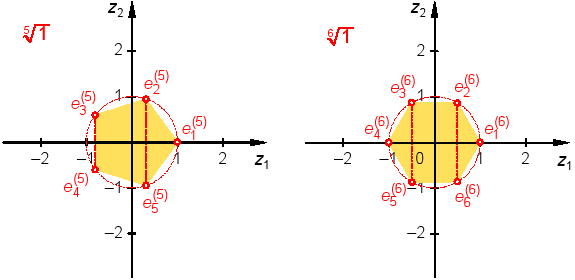
\includegraphics[width=7cm]{./bilder/einheitswurzel.png}
\end{minipage}

\vspace{-\baselineskip}
\subsection{12. Einheitswurzeln ($(k - 1) \cdot 30^{\circ}$)}
$e^{(12)}_1 = 1,\;
	e^{(12)}_2 = \frac{\sqrt3}{2} + \frac12j,\;
	e^{(12)}_3 = \frac12 + \frac{\sqrt3}{2}j,\;
	e^{(12)}_4 = j,\;
	e^{(12)}_5 = -\frac12 + \frac{\sqrt3}{2}j,\;
	e^{(12)}_6 = -\frac{\sqrt3}{2} + \frac12 j,\\
	e^{(12)}_7 = -1,\;
	e^{(12)}_8 = -\frac{\sqrt3}{2} - \frac12 j,\;
	e^{(12)}_9 = -\frac12 - \frac{\sqrt3}{2}j,\;
	e^{(12)}_{10} = -j,\;
	e^{(12)}_{11} = \frac12 - \frac{\sqrt3}{2}j,\;
	e^{(12)}_{12} = \frac{\sqrt3}{2} - \frac12j$

\subsection{Nullstellen von Polynomen}
Ein komplexes Polynom p(z) von Grad $n$ hat in $ \mathbb{C} $ genau $n$ Nullstellen.\\
Alle diese Nullstellen liegen in einer Kreisscheibe um den Ursprung mit dem Radius $r = \sum\limits_{k=0}^{n} \left| \frac{a_k}{a_n} \right| = \left| \frac{a_0}{a_n} \right| + \left| \frac{a_1}{a_n} \right| + ... + \left| \frac{a_n}{a_n} \right|$ \\ \\
Bei Polynomen mit reellen Koeffizienten treten nicht-reelle Nullstellen immer als konj.-kompl. Paare ($z_0$ und $\bar{z_0}$) auf.\\
Ein Polynom mit reellen Koeffizienten von \textit{ungeradem} Grad hat mind. eine \textit{reelle} Nullstelle.\\
Bei Polynomdivision immer mit reellen Zahlen arbeiten; konj.-kompl. Paare zusammenfassen.\\
\textbf{Berechnung:}\\
\begin{tabular}{l l}
	quadr. Polynome & Polynome mit $a_n = 1, a_{n-1} = a_{n-2} = ... = a_1 = 0, a_0 = a$\\
	$p(z) = az^2 + bz + c = 0$ & $p(z) = z^n + a = 0$\\
	$z_{1,2} = \frac{-b \pm \sqrt{b^2 -4ac}}{2a}$ & $z_k = \sqrt[n]{|a|} \cdot cjs(\frac{\varphi_a+\pi}{n} + (k-1) \cdot \frac{2\pi}{n})$ mit $k = 1, 2, ..., n$ 
\end{tabular}

\skriptsubsection{Euler}{30f}
\renewcommand{\arraystretch}{1.5}
\begin{tabular}{| l | l | l | l | l | l |}
\hline
	$\sin{\alpha} = \frac{e^{j\alpha} - e^{-j\alpha}}{2j}$ &

	$\cos{\alpha} = \frac{e^{j\alpha} + e^{-j\alpha}}{2}$ &

	$\tan{\alpha} = \frac{\sin \alpha}{\cos \alpha} = -j \frac{e^{j\alpha}-e^{-j\alpha}}{e^{j\alpha}+e^{-j\alpha}}$ & 

	$\sinh{\alpha} = \frac{e^\alpha - e^{-\alpha}}{2} $ &

	$\cosh{\alpha} = \frac{e^\alpha + e^{-\alpha}}{2} $ & 
	
	$\tanh{\alpha} = \frac{\sinh{\alpha}}{\cosh{\alpha}}$\\
\hline
\end{tabular}
\renewcommand{\arraystretch}{1}

\skriptsubsection{Überlagerung von harmonischen Schwingungen}{32f}
$$A \cdot \sin(\omega t + \varphi) = Im[A \cdot e^{j(\omega t + \varphi)}] =
Im[\underbrace{A \cdot e^{j\varphi}}_{\text{\tiny{Complexe Amplitude}}}
\cdot \underbrace{e^{j\omega t}}_{\text{\tiny{Zeitfunktion}}}]$$
%
%Alle komplexen Schwingungen in kartesische Form umwandeln und addieren, danach
%wieder zurück in Polarform $ A_{total} \cdot e^{j\varphi}$ zurückwandeln.
%
$$ A_1 \cdot \sin(\omega t + \varphi_1) + A_2 \cdot \cos(\omega t + \varphi_2) 
 \quad \Rightarrow \quad 
 Im[A_1 \cdot e^{j(\omega t + \varphi_1)} + A_2 \cdot e^{j (\omega t + \varphi_2
 + \frac{\pi}{2})}] \quad \Rightarrow \quad 
 Im[e^{j \omega t} \cdot  (A_1 \cdot e^{j \varphi_1} + A_2 \cdot e^{j (\varphi_2
 + \frac{\pi}{2})}]$$ 
Komplexe Amplituden in kartesische Form umwandeln, zusammenzählen und wieder
zurück in Polarform wandeln.
$$ Im[e^{j \omega t} \cdot  (A_{total} \cdot e^{j \varphi_{total}})] 
 \quad \Rightarrow \quad 
 Im[A_{total} \cdot e^{j (\omega t + \varphi_{total})}] 
 \quad \Rightarrow \quad 
 A_{total} \cdot \sin(\omega t + \varphi_{total})$$ 
$$A = |A_1 \cdot e^{j\varphi_1} + A_2 \cdot e^{j\varphi_2}| \qquad \varphi = arg(A_1 \cdot e^{j\varphi_1} + A_2 \cdot e^{j\varphi_2})$$

\skriptsection{Komplexe Funktionen (Abbildungen)}{37ff}
Eine komplexe Funktion hat einen 2-Dimensionalen Input ($z_1$, $z_2$) und einen
2-Dimensionalen Output ($w_1$, $w_2$). \\
Diese Abbildungen sind bis jeweils auf wenige Punkte (bei der Sinus-Funktion
$\pm$1, etc) winkeltreu.\\
$ f: \mathbb{D} \subseteq \mathbb{C} \mapsto \mathbb{C} \qquad z  \mapsto w = f(z) \qquad w_1 = \text{Re}(f(r+jc)); w_2 = \text{Im}(f(r+jc))$\\$
f'(z) = 0$ nicht winkeltreu! $\qquad f'(z) \neq 0$ winkeltreu! $\rightarrow$ Drehwinkel: $arg[f'(z)]$ und Streckfaktor: $|f'(z)|$
 

\skriptsubsection{Lineare Funktion}{41ff}
 	\begin{minipage}{9cm}
       $$ f : z \mapsto w = az + b \qquad (a, b \in \mathbb{C} \text{ und } a \neq0)\\$$
		- für $a = 1$ eine Translation um den Ortsvektor b \\
		- für $a \neq 1$ eine Drehstreckung mit dem Zentrum $\frac{b}{1-a}$, dem 
		Drehwinkel $\arg(a)$ und dem Streckfaktor $|a|$.  
    \end{minipage}
	\hspace{2cm}
	\begin{minipage}{8cm}
    	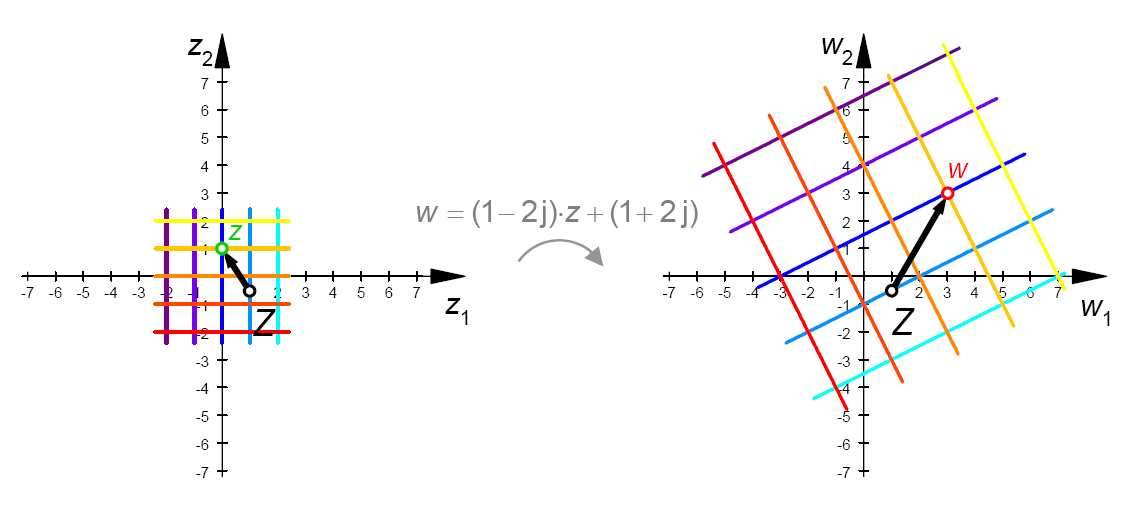
\includegraphics[width=8cm]{./bilder/LineareFunktion.png}
    \end{minipage}

\skriptsubsection{Quadratfunktion und Quadratwurzelfunktion}{45ff}
	\begin{minipage}{9cm}
    	$$ f : z \mapsto w = z^2 \qquad \qquad f : z \mapsto w = \sqrt{z} $$\\
		Bei der Quadratfunktion wird schon die rechte Hälfte der z-Ebene auf die ganze
		w-Ebene abgebildet (die Argumente werden verdoppelt). Mit der linken Hälfte zusammen ergeben sich
		zwei bzw. mehr Ebenen (Riemannsche Ebene).\\
		Sie ist überall Winkeltreu, ausser im Koordinatenursprung!
    \end{minipage}
	\hspace{2cm}
	\begin{minipage}{8cm}
    	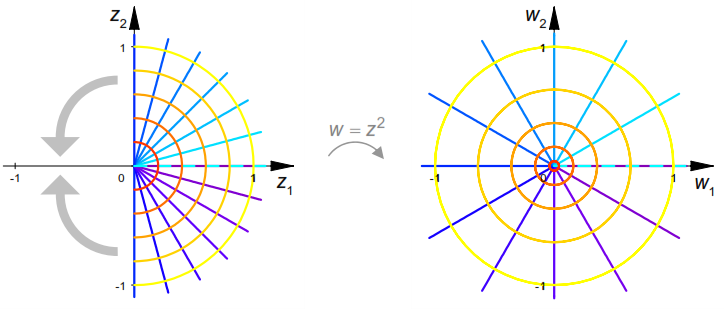
\includegraphics[width=8cm]{./bilder/quadrat.png} 
    \end{minipage}
    
\skriptsubsection{Sinus-Funktion}{67f}
	 \begin{minipage}{10cm}
		$$ f : z \mapsto w = \sin(z) $$    
		Die Sinusfunktion ist ausser bei den Punkten $z = \frac{\pi}{2}+ k\pi (k \in
		\mathbb{Z}))$ winkeltreu
	\end{minipage}
	\hspace{2cm}
	\begin{minipage}{7cm}
		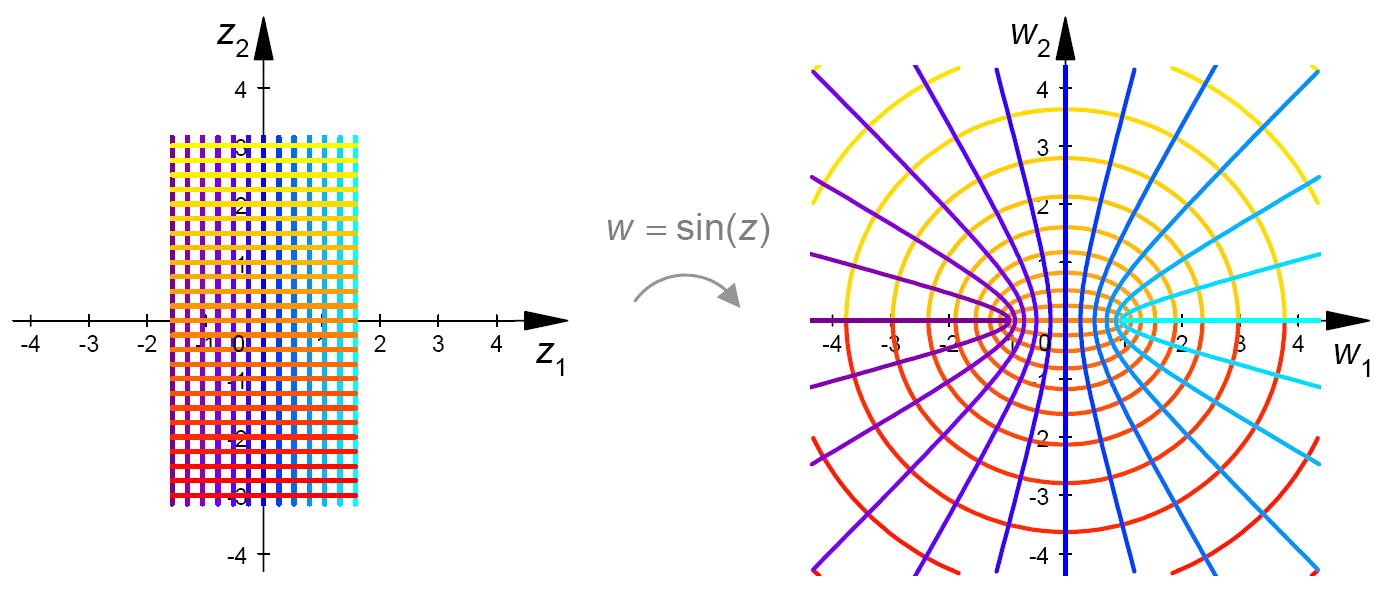
\includegraphics[width=7cm]{./bilder/sinus.png} 
	
	\end{minipage}

\skriptsubsection{Exponentialfunktion}{64ff} 
	\begin{minipage}{11cm}
		$$ f : z \mapsto w = e^z =e^{\text{Re}(z)}*\cjs(\text{Im}(z))$$
		Waagrechte Gitternetzlinen gehen gemäss der obigen Gleichung in Strahlen
		über, die im Koordinatenursprung beginnen, senkrechte Gitternetzlinien in
		Kreise um den Koordinatenursprung. Die e$^z$-Funktion ist periodisch, deshalb
		braucht es eine Riemannsche Fläche.\\ \\
		Mit dieser Funktion kann man das Feld an den Rändern des Plattenkondensators
		berechnen. 
	\end{minipage}
	\hspace{1cm}
	\begin{minipage}{7cm}
		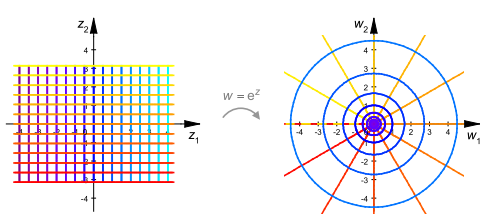
\includegraphics[width=7cm]{./bilder/exponentional.png} 		
	\end{minipage}
\skriptsubsection{Kehrwertfunktion und Kreisspiegelung}{51ff}
	$$\underbrace{f : z \mapsto w = \frac{1}{z};}_\text{Spiegelung an x-Achse (Kehrwert)} \quad (\arg(w) = -\arg(z), |w| = \frac{1}{|z|})
	\qquad \qquad 
	\underbrace{\overline{f}: z \mapsto w = \frac{1}{\overline{z}};}_\text{Kreisspiegelung}  \quad  
	(\arg(w) = \arg(z), |w| = \frac{1}{|z|}) $$
	\begin{tabbing}
		xxxx\=xxxxxxxxxxxxxxxxxxxxxxxxxxxxxxxxxxxxxxxxxxxxxxxxxxxxxxxxxx\=xxxxxxx\kill
		\> überall ausser im Ursprung winkeltreu \> überall winkeltreu
	\end{tabbing}


	\begin{minipage}{9cm}
		Kreisspiegelung: Alle Punkte auf der z-Ebene werden am Einheitskreis gespiegelt.
		Geraden auf Kreise abgebildet und umgekehrt. Der Ursprungspunkt (0;0) wird auf
		$ \infty $ abgebildet (auf allen Winkeln zwischen $0^o-360^o$). Die
		Abbildungen sind im verallgemeinerten Sinn (Geraden sind Kreise mit unendlichem Radius)
		kreistreu. Ausserdem sind sie, auch im Koordinatenursprung, winkeltreu.\\
		\begin{tabbing}
        	xxxxxxxxxxxxxxxxxxxxxxx\=xxxxxxxxxxxxxxxxxxxxxxxx\kill
	        - Gerade durch 0 $\Longrightarrow$ \>Fixgerade (gleiche Gerade, aber
	        die \\ \>Punkte darauf sind anders verteilt)\\ \\
			- Gerade nicht durch 0 $\Longrightarrow$ Kreis durch 0\\ \\ 
			- Kreis nicht durch 0 $\Longrightarrow$ \>Spiegelung des Kreises\\ \> am Einheitskreis\\ \\
			- Kreis durch 0 $\Longrightarrow$\>Gerade nicht durch 0
        \end{tabbing}
	\end{minipage}
	\hspace{2cm}
	\begin{minipage}{6cm}
		%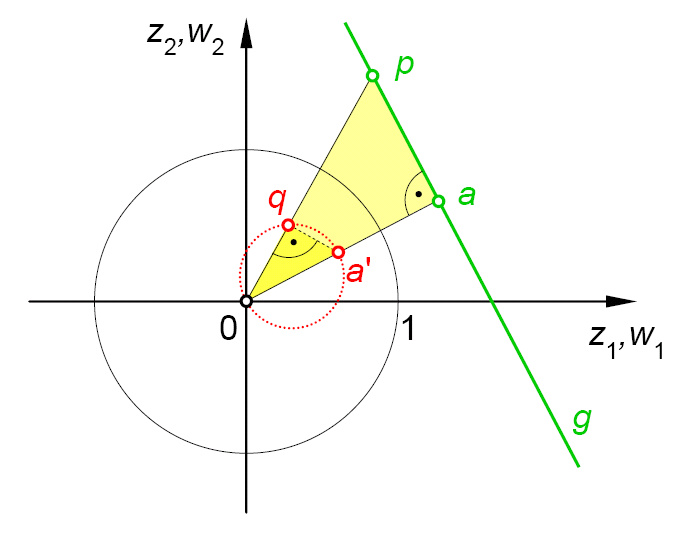
\includegraphics[width=6cm]{./bilder/GeradeKreisspiegelung.png} 
    		%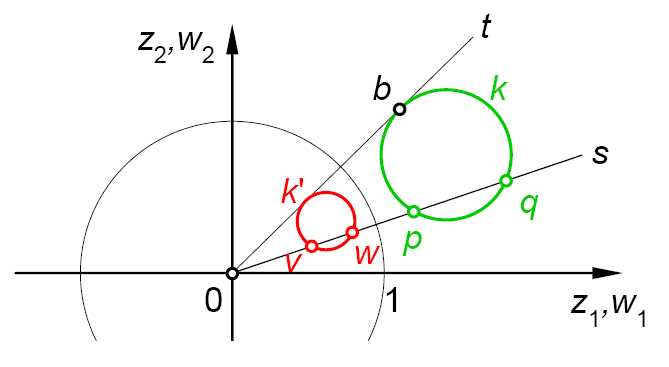
\includegraphics[width=6cm]{./bilder/KreisKreisspiegelung.png}
		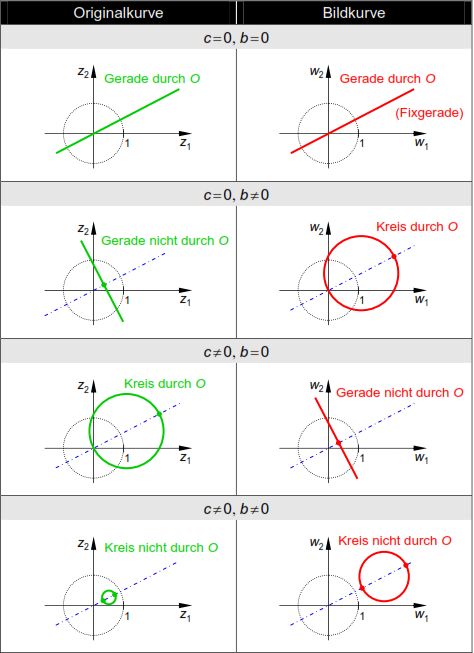
\includegraphics[width=6cm]{./bilder/Kurvenspiegelung.png}
    \end{minipage}


%\skriptsubsection{Möbiustransformation}{57ff}
%	\begin{minipage}{10cm}
%		$$ f : z \mapsto w = f(z) = \frac{az + b}{cz + d}$$
%		$$(a, b, c, d \in 
%		\mathbb{C} \text{ mit } c \neq 0 \text{ und } ad - bc \neq 0) $$
%		Die Möbiustransformation ist eine Verkettung einer linearen Funktion, der Kehrwertfunktion und einer weiteren linearen Funktion. \\
%		Diese Transformationen sind winkel- und kreistreu. Die Umkehrfunktion ergibt wieder eine Möbiustransformation. \\
%		Eigentlich besitzt diese Funktion nur drei Parameter da man den Bruch
%		$\frac{az + b}{cz + d}$ stets so kürzen kann dass einer der vier Parameter 1
%		ist. Durch die 3 Freiheitsgrade kann man unterschiedlichste kriterien
%		vorgeben und damit komplizierte Umformungen machen, wie im Bild gezeigt wird:
%	
%	\end{minipage}
%	\hspace{2cm}
%	\begin{minipage}{7cm}
%		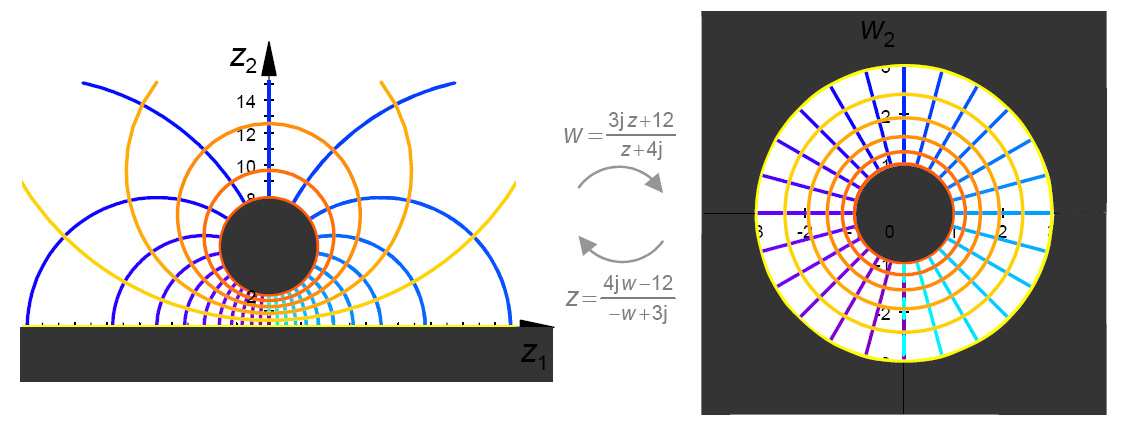
\includegraphics[width=7cm]{./bilder/Moebiustransformation.png} 
%	\end{minipage}
%
%\skriptsubsection{Joukowski-Funktion}{60ff}
%	\begin{minipage}{10cm}
%		$$ f : z \mapsto w = z + \frac{1}{z}  $$
%		Die Funktion ist winkeltreu bis auf $\pm$2\\
%		Wenn man einen Kreis, der nicht ganz im Zentrum steht transformiert ergibt
%		sich ein Flügelprofil
%	\end{minipage}
%	\hspace{2cm}
%	\begin{minipage}{7cm}
%		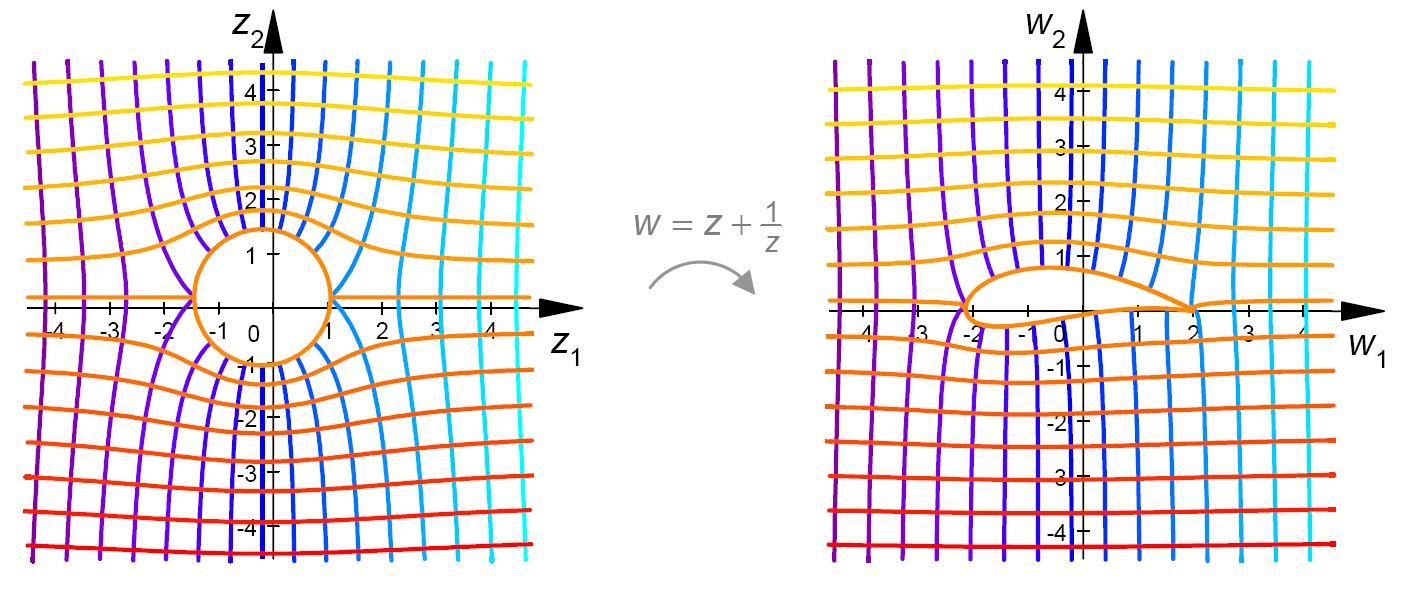
\includegraphics[width=7cm]{./bilder/joukowskiFunktion.png} 
%
%	\end{minipage}
 
\subsection{Kreisgleichung}
Die Lösungen von z bilden einen Kreis mit dem Radius $r$ um den Mittelpunkt $M=(m_x, m_y) \Rightarrow m=m_x + j m_y$. \\
$$|z-m| = r; \qquad 
(z-m)(\overline{z} - \overline{m}) = r^2; \qquad 
z\overline{z} - \overline{m}z - m\overline{z} + m\overline{m} = r^2$$
$$ \text{Parameterform: } f(t) = m + r \cdot e^{jt}, \quad \text{mit } (0 \leq t \leq 2 \pi) $$

\skriptsection{Fourierreihen}{70ff}
    \skriptsubsection{Orthogonalitätsbeziehungen der Basisfunktionen}{75}
        \begin{tabular}{lll}
            $\int\limits_0^T \cos(n\omega t)\cdot \cos(m\omega t)dt=
            \begin{cases}
            T$ für $n=m=0\\
            \frac{T}{2},$ für $n=m>0\\ 
            0,$ für $n\neq m\\
            \end{cases}$ &
            $\int\limits_0^T \sin(n\omega t)\cdot \sin(m\omega t)dt=
            \begin{cases}
            \frac{T}{2},$ für $n=m\\
            0,$ für $n\neq m\\
            \end{cases}$&
            $\int\limits_0^T \cos(n\omega t)\cdot \sin(m\omega t)dt=0$\\

	$(m,n \in \mathbf{N_0})$ &
	$(m,n \in \mathbf{N})$ &
	$(m \in \mathbf{N_0} ; n \in \mathbf{N})$
        \end{tabular}

	\skriptsubsection{Allgemeine Form}{79}
		Eine periodische Funktion f mit Periode $T>0$, lässt sich durch eine Reihe von
		Sinus- und Kosinusfunktionen darstellen, deren Frequenzen ganzzahlige 
		Vielfache der Grundfrequenz $\omega = 2\pi / T$ sind:
		$$ FR[f(t)] = f(t) =\frac{a_0}{2} + \sum_{n=1}^\infty (a_n \cdot \cos(n \omega t) + b_n
		\cdot \sin(n\omega t))$$
		Die Koeffizienten der Entwicklung von $f(t)$ sind:
		$$ a_n=\frac{2}{T}\int_{0}^{T} f(t) \cdot \cos(n\omega t)\, \mathrm{d}t \quad (n=0,1,2,3,\ldots)
		 \qquad \qquad b_n=\frac{2}{T}\int_{0}^{T} f(t) \cdot \sin(n\omega t)\,
		 \mathrm{d}t \quad (n=1,2,3,\ldots) $$ 
		Der erste Summand der Reihe $a_0/2$ ist der Gleichstromanteil (Mittelwert) von
		$f(t)$ im Intervall $(0,T)$
		$$ a_0=\frac{2}{T}\int_{0}^{T} f(t)\ \mathrm{d}t \quad (n=0)$$

	\skriptsubsection{Komplexwertige Darstellung der Fourierreihen}{95ff}
		$$f(t) = \sum\limits_{k = -\infty}^{\infty} c_k \cdot e^{j k \omega t} \qquad \text{mit} \qquad c_n=\overline{c_{-n}}=\frac{1}{T}\int_0^T{f(t)\cdot e^{-jn\omega t}dt} \qquad (n \in \mathbf{N_0})$$
		\subsubsection{Umrechnungsformeln}
			$$c_n=\overline{c_{-n}}=\frac{a_n-jb_n}{2} (n=0,1,2,3,\ldots\text{ wobei }b_0=0)\qquad
			\left.
			\begin{array}{l} 
				a_n=2Re(c_n) = c_n + c_{-n}\\
				b_n=-2Im(c_n) = j(c_n - c_{-n})
			\end{array}
		    \right\} 
		    \quad \begin{array}{l}
				(n \in \mathbf{N_0}) \\
				(n \in \mathbf{N})
			\end{array}$$ \\
		$c_0 = \frac{a_0}{2} \qquad c_{-n} = \frac{a_n + jb_n}{2}$

	  
	\skriptsubsection{Sätze zur Berechnung der Koeffizienten}{80ff}
		\skriptsubsubsection{Symmetrie}{78}
		Allgemein:$\qquad$ gerade $\cdot$ ungerade $=$ ungerade; $\qquad$ ungerade $\cdot$ ungerade $=$ gerade $\cdot$ gerade $=$ gerade

		\begin{tabular}{l l l l l}
   			Falls $f(t)$ \textbf{gerade} ($ f(-t)=f(t) $) ist &
   			$\Longrightarrow$ & 
			$b_n = 0,$ &
			$a_n = \frac{4}{T} \int\limits_0^{\frac{T}{2}} f(t) \cdot \cos(n \omega t) \mathrm{d}t$ &
			$Im[c_n] = 0$ \\
			
			& & \multicolumn{3}{l} {(achsensymmetrisch: Spiegelung an Y-Achse)}\\
			& & \multicolumn{3}{l} {wenn $f(t)$ gerade ist bezgl. $\frac{T}{4} \Rightarrow a_{2m+1} = 0$}\\
			& & \multicolumn{3}{l} {wenn $f(t)$ ungerade ist bezgl. $\frac{T}{4} \Rightarrow a_{2m} = 0$}\\

			Falls $f(t)$ \textbf{ungerade} ($ f(-t)=-f(t) $) ist &
			$\Longrightarrow$ &
			$a_n = 0,$ &
			$b_n =  \frac{4}{T}\int\limits_0^{\frac{T}{2}} f(t) \cdot \sin(n \omega t) \mathrm{d}t$ &
			$ Re[c_n] = 0$\\

			& & \multicolumn{3}{l} {(punktsymmetrisch: Punktspiegelung im Ursprung)}\\
			& & \multicolumn{3}{l} {wenn $f(t)$ gerade ist bezgl. $\frac{T}{4} \Rightarrow b_{2m} = 0$}\\
			& & \multicolumn{3}{l} {wenn $f(t)$ ungerade ist bezgl. $\frac{T}{4} \Rightarrow b_{2m+1} = 0$}\\
      	\end{tabular}
			 
		\skriptsubsubsection{Linearität}{81}
			$h(t) = r \cdot f(t) + s \cdot g(t) \quad \Longrightarrow \quad a_n^{(h)} = r \cdot
			a_n^{(f)} + s \cdot a_n^{(g)}, \quad b_n^{(h)} = r \cdot b_n^{(f)} + s \cdot b_n^{(g)} \qquad f$, $g$ und $h$ sind T-periodische Funktionen
			
		\skriptsubsubsection{Zeitstreckung/-stauchung ("Ahnlichkeit)}{82}
			$g(t) = f(r \cdot t) $ (mit $ 0 < r \in \mathbb{R}$ ) $\quad \Longrightarrow\quad  
			a_n^{(g)} = a_n^{(f)}, \quad b_n^{(g)} = b_n^{(f)} $ \quad $T^{(g)} = \frac{T^{(f)}}{r} \qquad \omega_g = \frac{2\pi}{T_g}\qquad r\flq1:$Streckung$; r\frq1: $Stauchung
			Zeitspiegelung: $g(t) = f(-1\cdot t) \Longrightarrow \quad a_n^{(g)}=a_n^{(f)}, \quad b_n^{(g)} = sgn(-1)\cdot b_n^{(f)} \qquad $
			
		\skriptsubsubsection{Zeitverschiebung}{84} 
		\label{Fourier_Zeitverschiebung}
		$g(t)=f(t+t_0)$
		$\qquad
		\begin{array}{l}
           a_n^{(g)}=\cos(n\omega t_0)\cdot a_n^{(f)}+\sin(n\omega t_0)\cdot b_n^{(f)}\\
           b_n^{(g)}=-\sin(n\omega t_0)\cdot a_n^{(f)}+\cos(n\omega t_0)\cdot b_n^{(f)}\\
           c_k^{(g)}=e^{jk \omega t_o} \cdot c_k^{(f)}
        \end{array}$
        $\quad
		\begin{array}{l}
           (n=0,1,2,\ldots)  \qquad \text{mit }b_0 = 0 \qquad\\
           (n=1,2,3,\ldots)\\
           (k \in \mathbb{Z})
        \end{array}$
    	$\quad
    	\begin{array}{l}
    		 +t_0$: links$\\
    		  -t_0$: rechts$
    	\end{array}
    	$

\begin{multicols}{2}
	\skriptsubsection{Satz von Dirichlet}{89}
	Die Funktion $f(t)$ sei $T$-periodisch und stückweise stetig mit Limes, dann konvergiert ihre Fourierreihe gegen\\
	$$FR[f(t_0)] = f(t_0) = \frac{f(t_{0-}) + f(t_{0+})}{2}$$
	somit in die Mitte einer Sprungstelle oder den Funktionswert selber.
\vfill\null
\columnbreak
	\skriptsubsection{Abstand f - g}{84}
	Abstand zweier $T$-periodischen, mit Limes stückweise stetigen Funktionen $f$ und $g$.
	$$||f - g|| = \sqrt{\frac{2}{T}\int\limits_0^2[f(t) - g(t)]^2 \mathrm dt} $$
\vfill\null
\end{multicols}

\begin{multicols}{2}
\skriptsubsection{Parsevalsche Gleichung}{97}
$$\frac{a_0^2}{2} + \sum_{n=1}^{\infty}(a_n^2+b_n^2) = \frac{2}{T}\int_{0}^{T}[f(t)]^2dt = ||f||^2$$
$$\sum\limits_{k = -\infty}^{\infty}|c_k|^2 = \frac{1}{T}\int\limits_{0}^{T}[f(t)]^2\mathrm dt$$
\vfill\null
\columnbreak		
\skriptsubsection{Integral und Differential}{88}
Falls die T-periodische Funktion $f$ (auf ganz $\mathbb{R}$) zweimal stetig differenzierbar ist und die Fourierkoeffizienten $a_n$ und $b_n$ besitzt, so gilt:
$$ f'(t) = \sum\limits_{n=1}^{\infty} [b_n n \omega \cdot \cos{(n \omega t)} - a_n n \omega \cdot \sin{(n \omega t)}]$$
$$\int\limits_0^t f(\tau) d\tau = \sum\limits_{n=1}^{\infty} [\frac{b_n}{n \omega}] + 
\frac{a_0}{2} t + \sum\limits_{n=1}^{\infty}
[\frac{a_n}{n \omega} \cdot \sin{(n \omega t)} - \frac{b_n}{n \omega} \cdot \cos{(n \omega t)}] $$
\end{multicols}

\skriptsubsection{Gibbs'sches Phänomen}{92f}
\begin{figure}[htbp]
	\vspace{-\baselineskip}
	\begin{minipage}[c]{8cm}
		Die Fourierreihen schwingen bei Unstetigkeitsstellen über. Die Höhe der grössten überschwingenden Welle
		beträgt 8.94\% der gesamten Sprunghöhe.
	\end{minipage}
	\begin{minipage}[c]{8cm}
		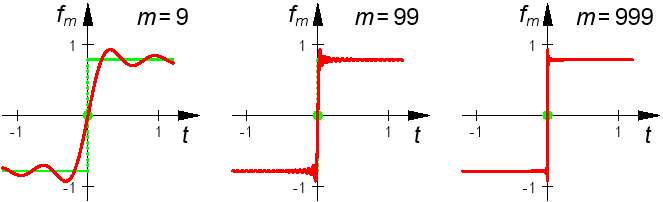
\includegraphics[width=8cm]{./bilder/gibssches_phaenomen.png}  
	\end{minipage}
\end{figure}
\vspace{-\baselineskip}

\skriptsection{Spektren}{103}
\begin{minipage}{0.3\linewidth}
	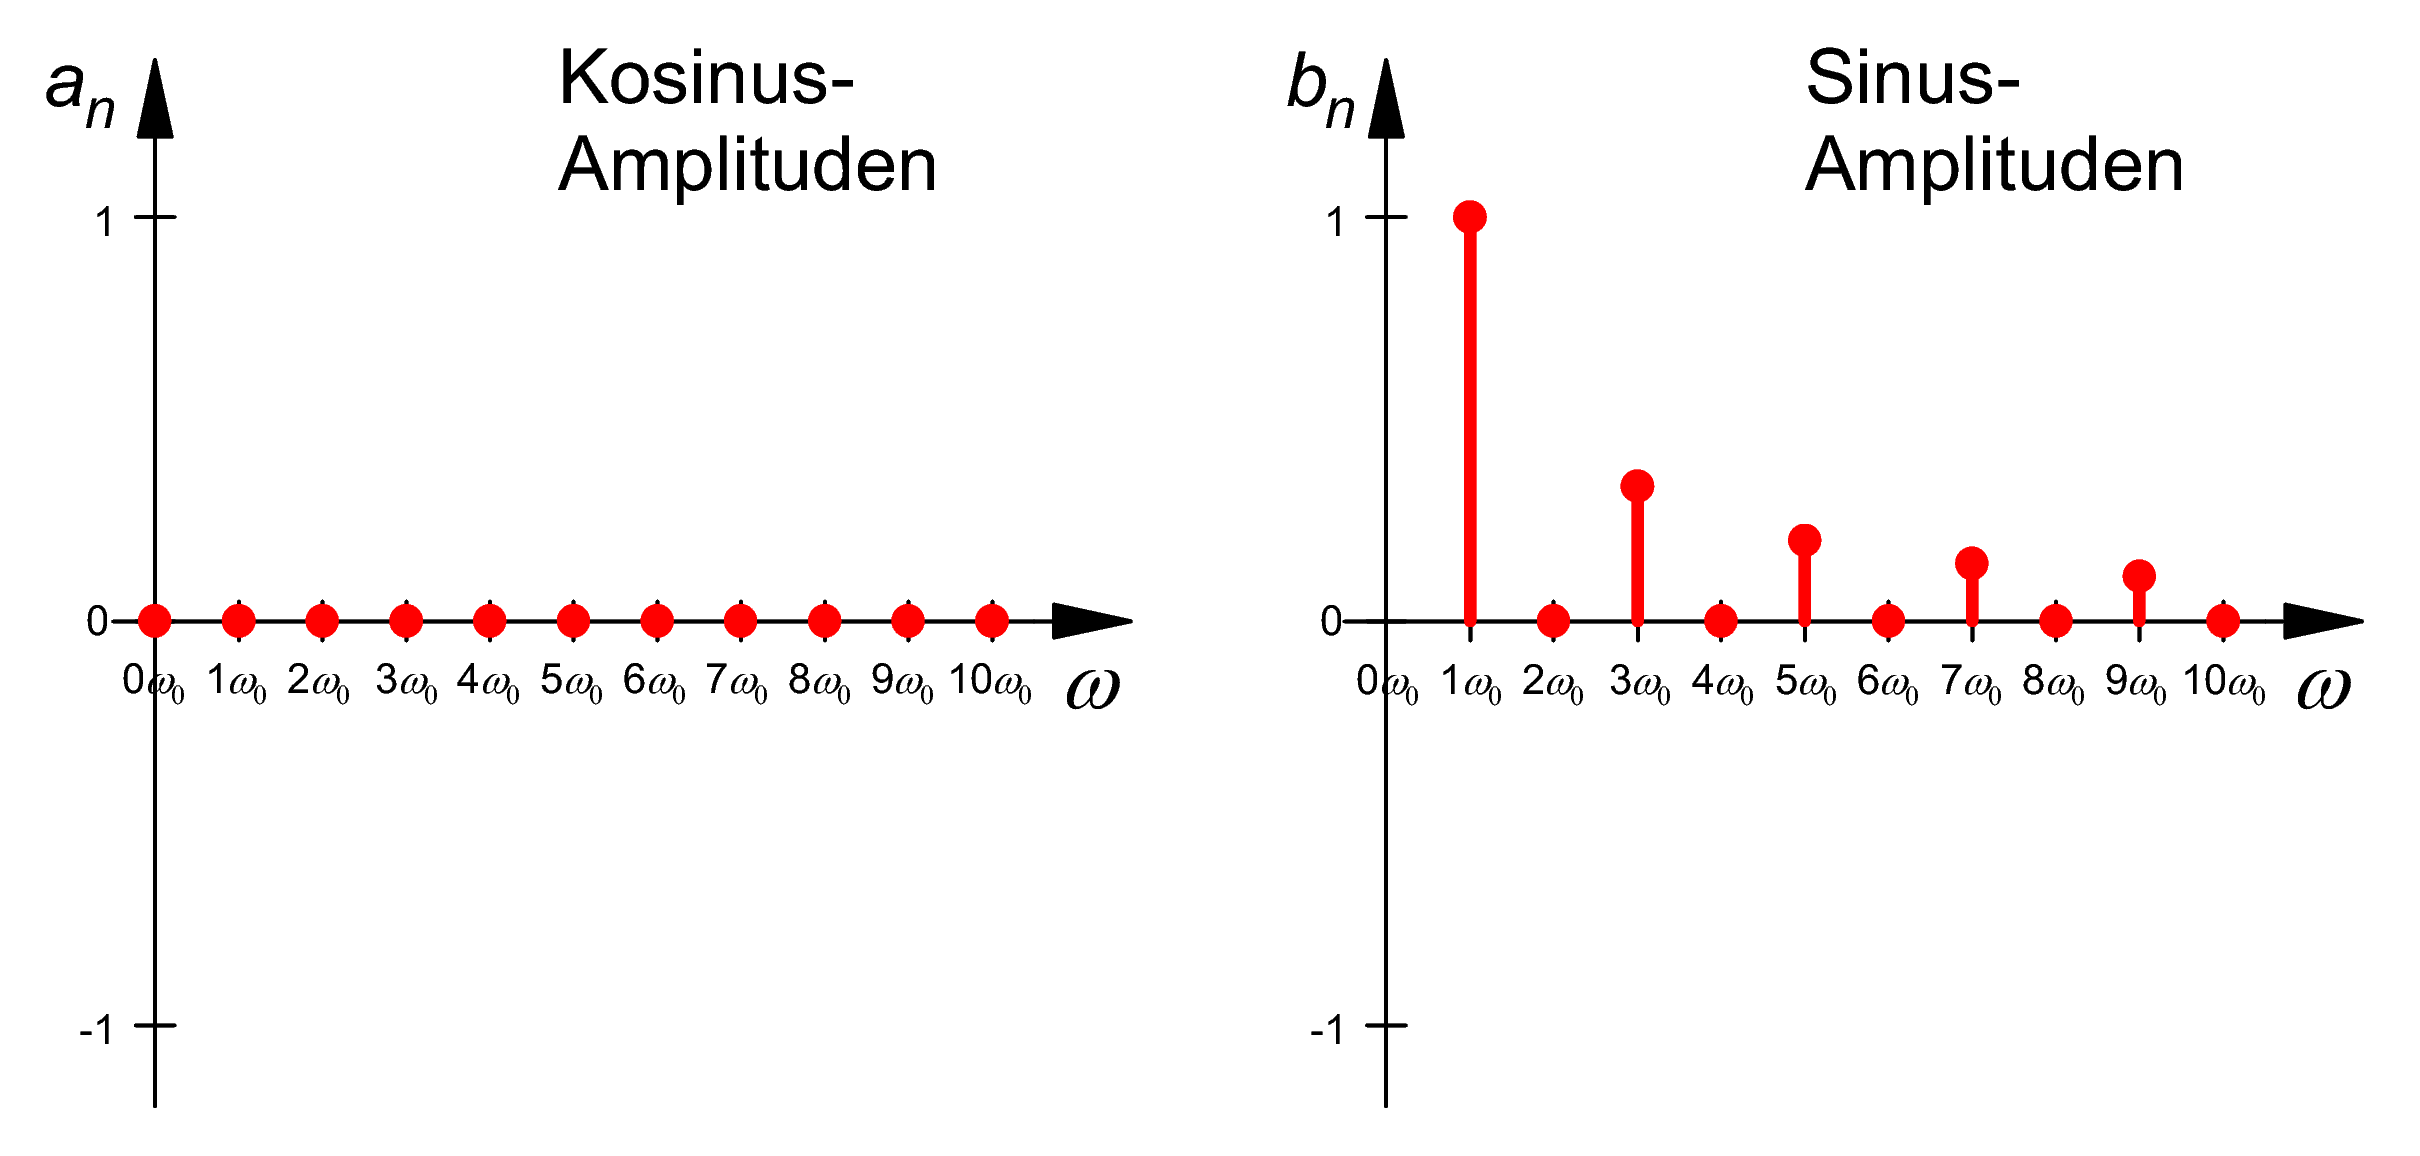
\includegraphics[width=\linewidth]{./bilder/spektren_cossin.png}
	\small{Kosinus- und Sinusamplitudendiagramm}
\end{minipage}%
\hspace{0.01\linewidth}
\begin{minipage}{0.31\linewidth}
	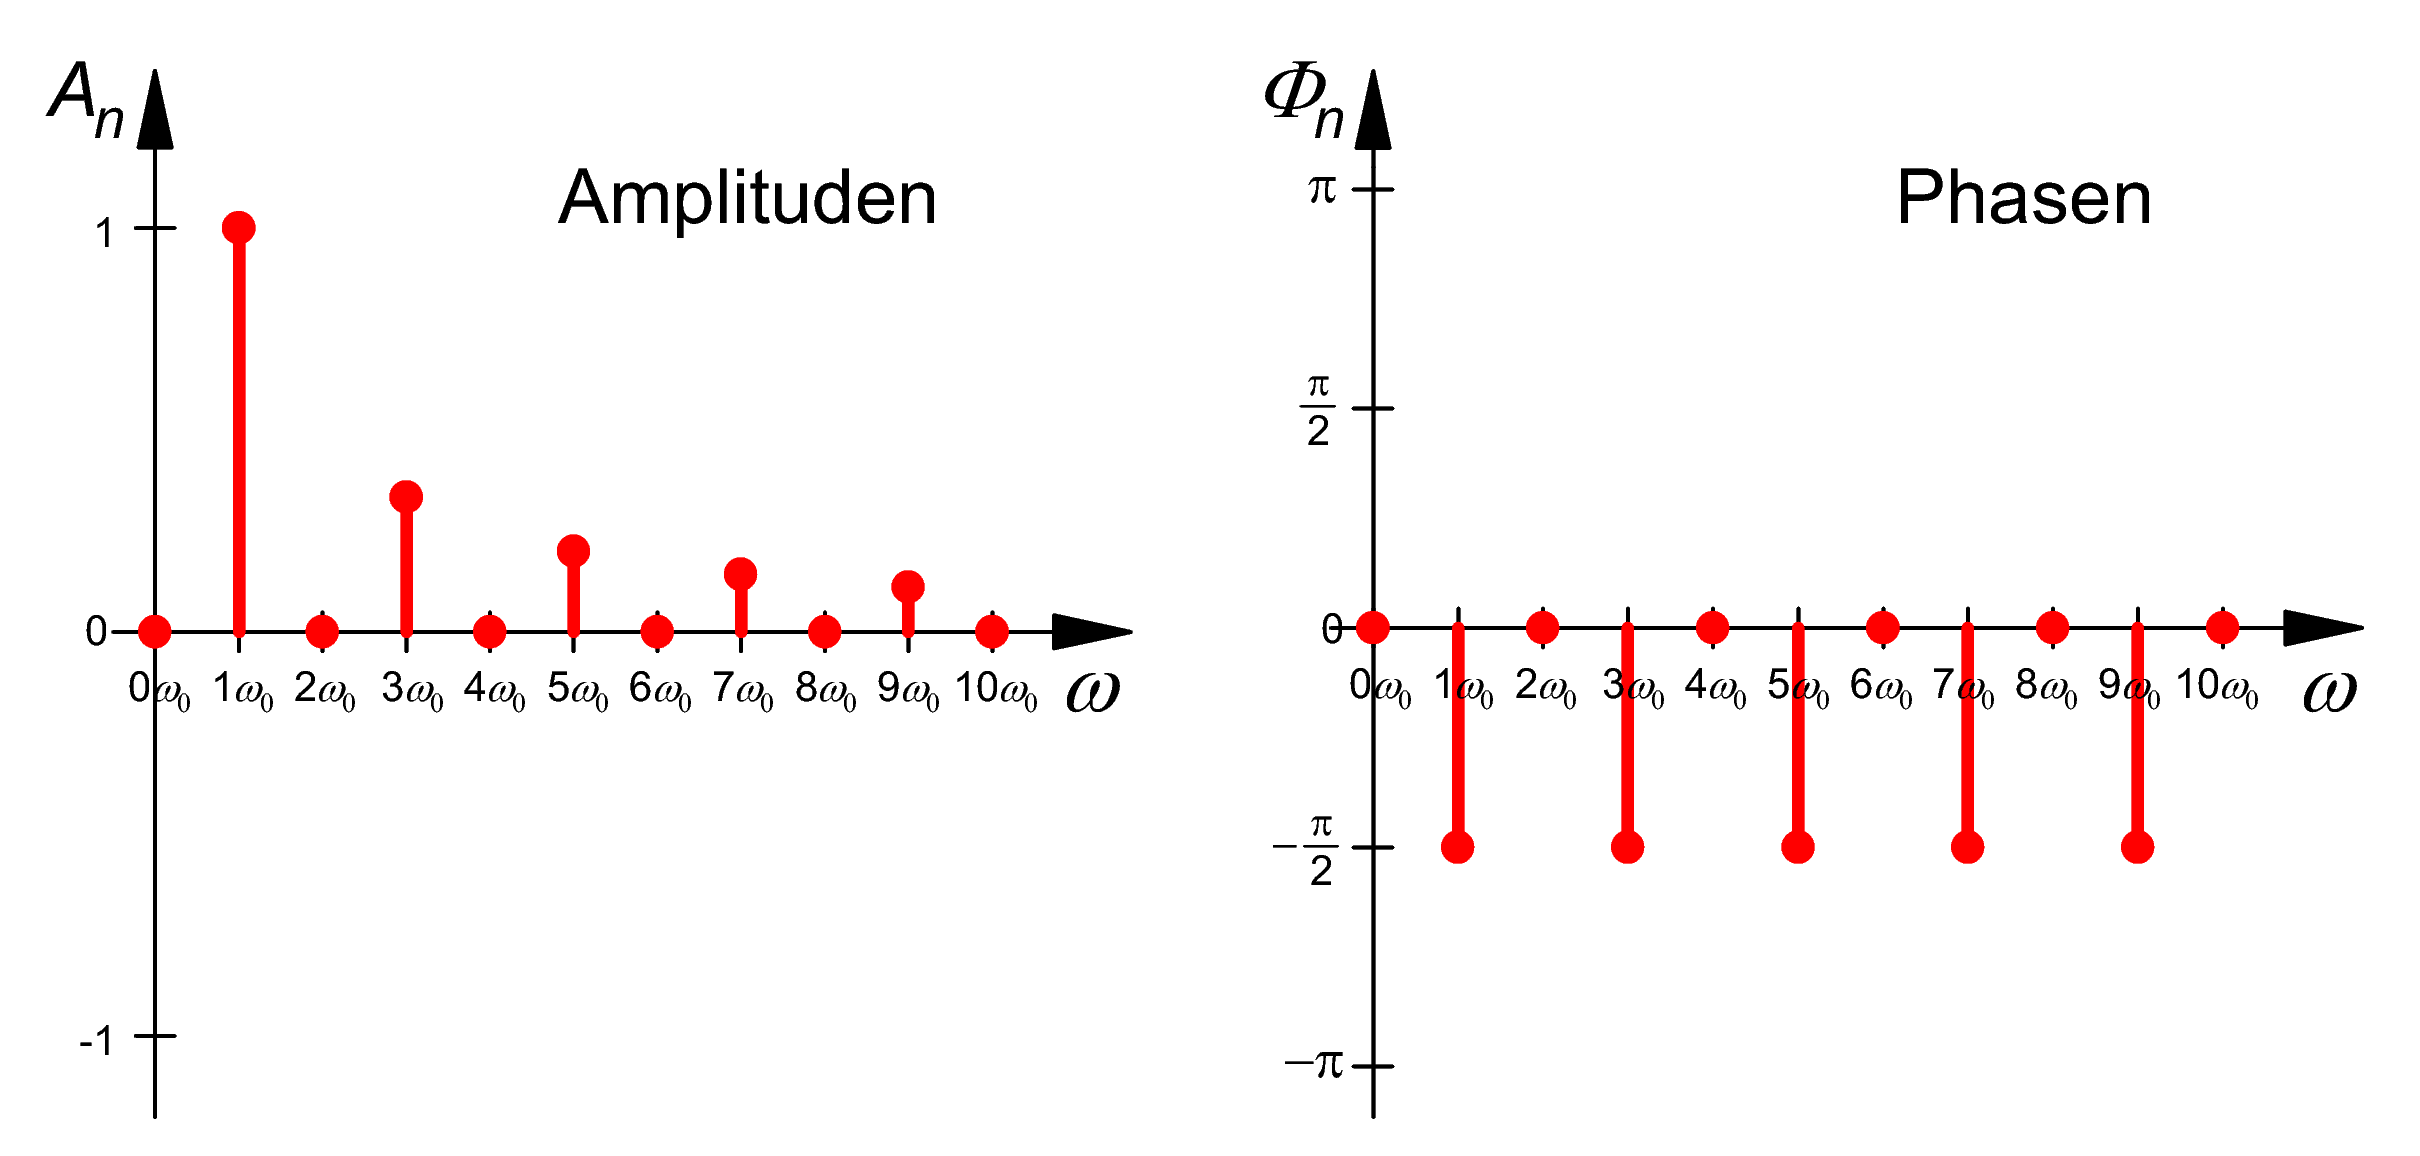
\includegraphics[width=\linewidth]{./bilder/spektren_einseitig.png}
	\small{1-seitiges Amplituden-/Phasendiagramm}
\end{minipage}%
\hspace{0.01\linewidth}
\begin{minipage}{0.31\linewidth}
	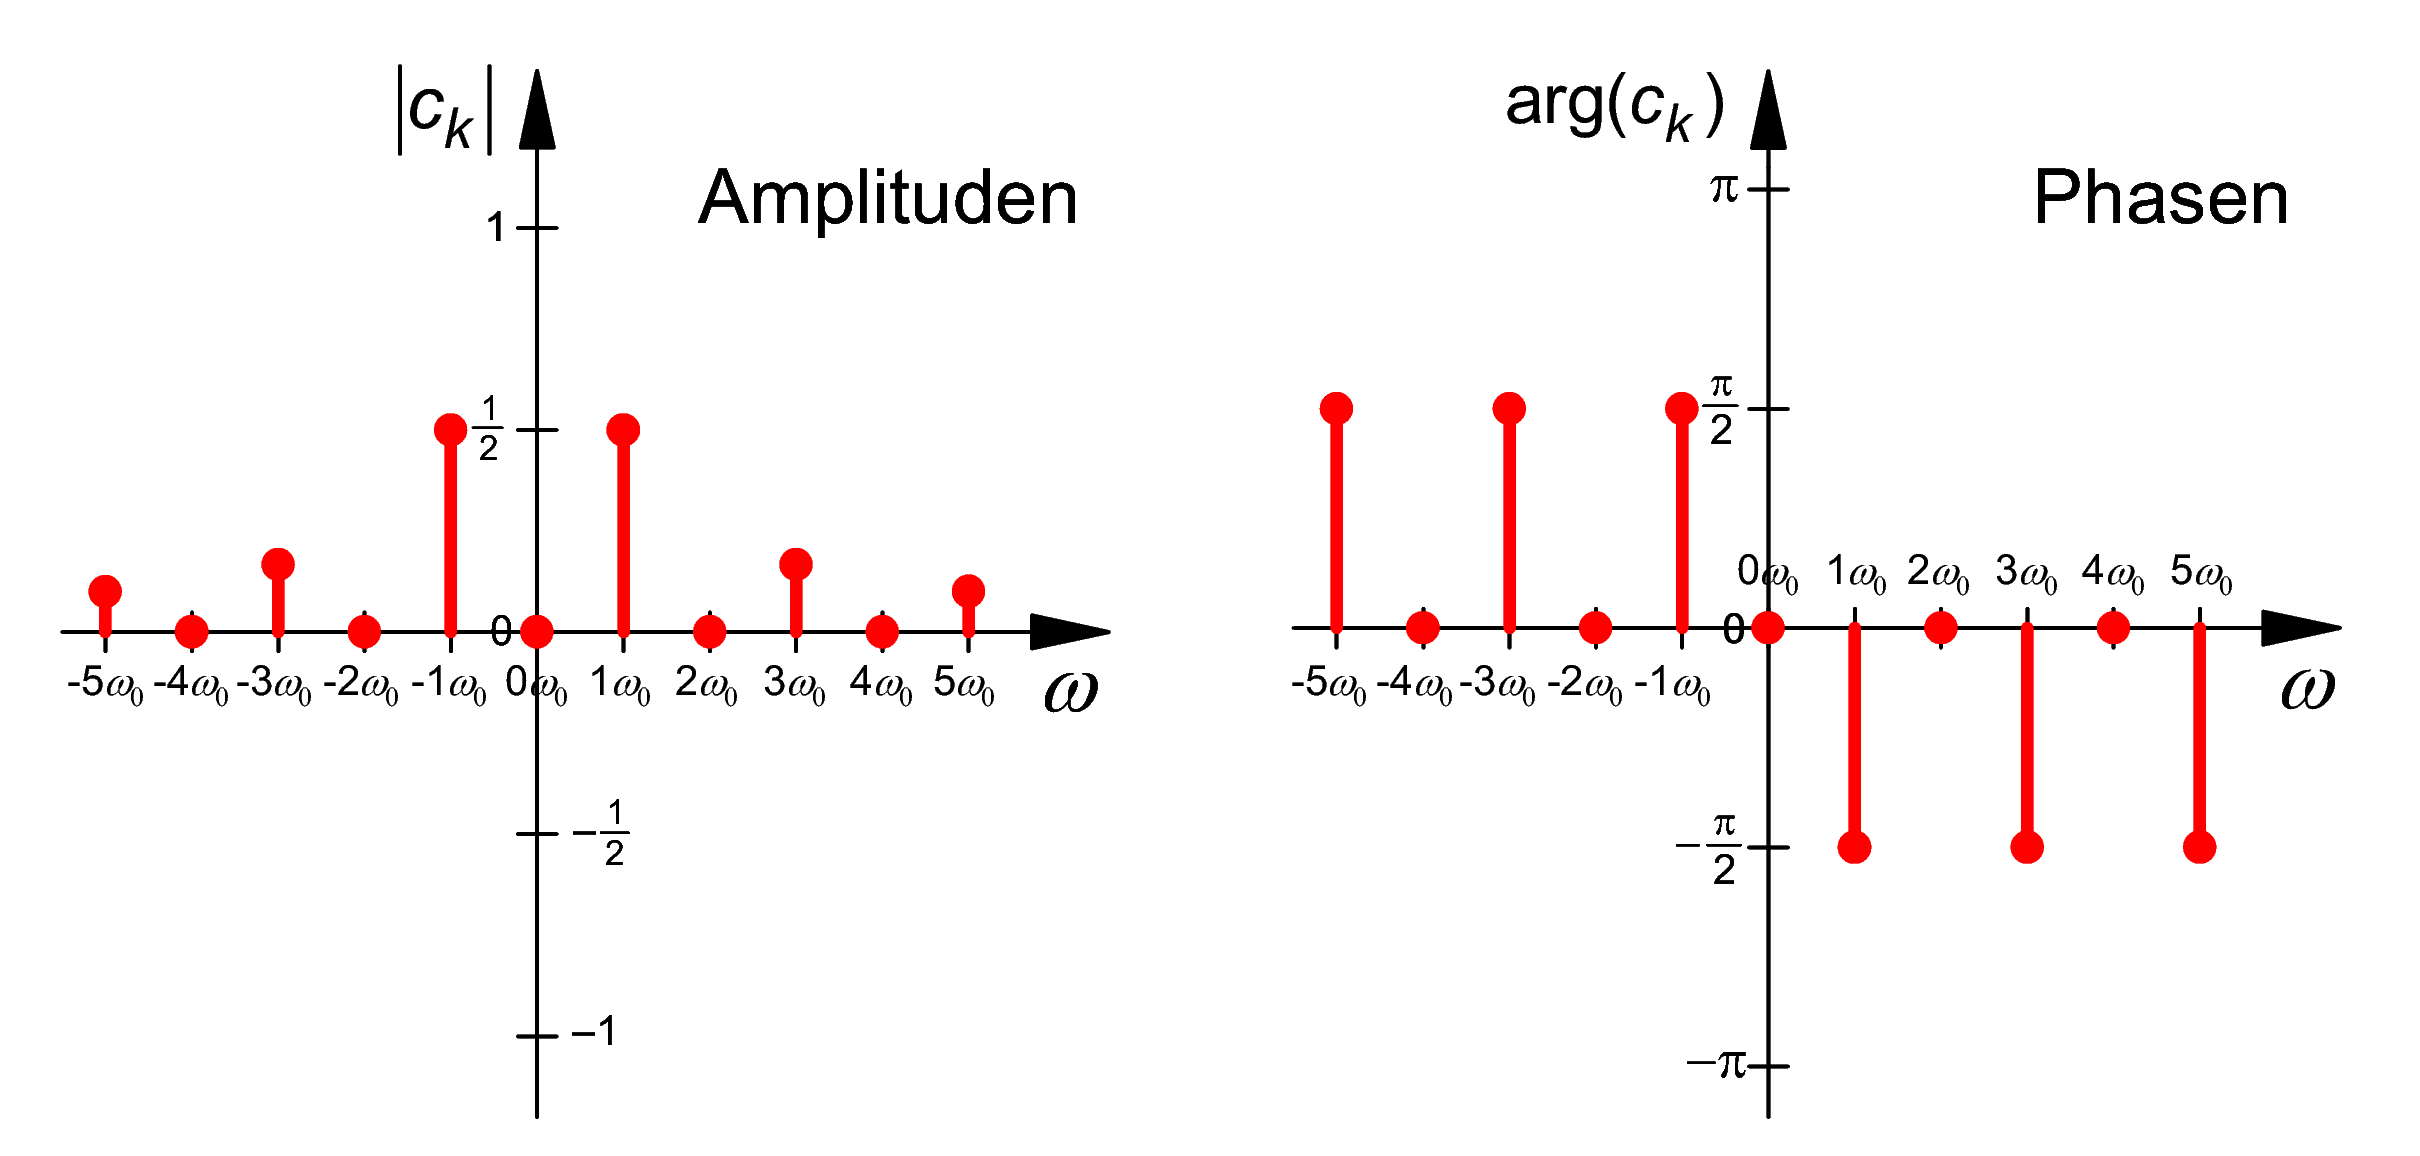
\includegraphics[width=\linewidth]{./bilder/spektren_zweiseitig.png}
	\small{2-seitiges Amplituden-/Phasendiagramm}
\end{minipage}

\subsubsection{(1) Kosinus- und Sinusamplitudendiagramm} 
Reelle Fourierkoeffizienten ($a_n, b_n$) können direkt abgelesen werden. 
Bei einer Phasenverschiebung ändern sich jedoch die Koeffizienten grafisch nicht nachvollziehbar. \\
Diese Darstellung hat gegenüber den anderen mehr Nachteile und wird daher eher selten genutzt.

$$a_n = A_n \cdot \cos(\varphi_n) = 2\cdot Re(c_n) \qquad b_n = -A_n \cdot \sin(\varphi_n) = A_n \sin(-\varphi_n) = -2\cdot Im(c_n)$$

\begin{multicols}{2}
	\subsubsection{(2) Einseitiges Amplituden-/Phasendiagramm} 
	$A_n = |a_n - j \cdot b_n| = \sqrt{a_n^2 + b_n^2}$ oder $A_n = 2 \cdot |c_n|$\\
	$\varphi_n = \arg(a_n - j \cdot b_n) = \arctan(-\frac{b_n}{a_n}) \text{ oder } \varphi_n = \arg(c_n) $ \\
	Spezialfall $n=0 \Rightarrow A_0 = |\frac{a_0}{2}| \text{ und } \varphi_0 = \left\{
	\begin{array}{l} 
	0, \quad a_0 \geq 0\\
	\pi, \quad a_0 < 0  
	\end{array}
	\right. $\\
	\vfill\null
	\columnbreak
	\subsubsection{(3) Zweiseitiges Amplituden-/Phasendiagramm}
	\textbf{(komplexes Spektrum)}\\ 
	Amplitudendiagramm ist achsensymmetrisch weil $ c_n=\overline{c_{-n}} $. Phasendiagramm ist punktsymmetrisch. \\
	Ähnlichkeit mit Einseitigem: $|c_n| = \frac{1}{2}A_n $ und $\varphi_n$ gleich wie bei (2) für alle $ n \geq 0$.\\
	$A_0 = |\frac{a_0}{2}| = |c_0| $
	$$arg(c_{-n}) = -arg(c_n) \qquad c_n = \frac{a_n - jb_n}{2} \qquad \varphi_n = arg(a_n - jb_n) \qquad c_n = \frac{A_n}{2} \cdot e^{j\varphi_n}$$
\end{multicols}

\skriptsubsection{Spezialfälle}{106}
\begin{tabular}{ll}
	Funktion f gerade 
	& (1) Sinusphasendiagramm überall 0 \\
	& (2,3) Phasendiagramm enthält nur die Werte $0$ und $\pi$ \\
	Funktion f ungerade
	& (1) Kosinusphasendiagramm überall 0 \\
	& (2,3) Phasendiagramm enthält nur die Werte $\pm \frac{\pi}{2}$ (oder $0$ falls Amplitudenwert $=0$) \\
	"Ahnlichkeit $g(t) = f(r \cdot t) $
	& (1,2,3) Das Spektrum von $g$ ist das horizontal mit den Faktor $r$ gestreckte Spektrum vom $f$. \\
	Zeitverschiebung $g(t) = f(t + t_0) $
	& (1) \verweis{Fourier_Zeitverschiebung}{Zeitverschiebung} \\
	& (2,3) Amplitudendiagramme sind identisch. \\
	& (2,3) Phasendiagramme: Die Sälule der Frequenz $k \omega_0$ wächst um $k\omega_0 t_0$. \\
	Weisses Rauschen
	& "Uberlagerung von Schwingungen aller möglichen Frequenzen \\
	& mit gleichen Amplituden und zufälligen Phasen. 
\end{tabular}
\vspace{-\baselineskip}
\label{LastPage}
\section{Wichtige Formeln}	
\subsection{Funktionswerte für Winkelargumente}
\renewcommand{\arraystretch}{1.5}
\begin{minipage}{5cm}
	\begin{tabular}[c]{ |c|c||c|c|c| }
		\hline
		deg & rad & sin & cos & tan\\
		\hline
		0\symbol{23} & 0 & 0 & 1 & 0\\
		\hline
		30\symbol{23} & $\frac{\pi}{6}$ & $\frac{1}{2}$ & $\frac{\sqrt{3}}{2}$ &
		$\frac{\sqrt{3}}{3}$\\
		\hline
		45\symbol{23} & $\frac{\pi}{4}$ & $\frac{\sqrt{2}}{2}$ & $\frac{\sqrt{2}}{2}$
		& 1\\
		\hline
		60\symbol{23} & $\frac{\pi}{3}$ & $\frac{\sqrt{3}}{2}$ & $\frac{1}{2}$ &
		$\sqrt{3}$\\
		\hline			
	\end{tabular}			
\end{minipage}
\begin{minipage}{4.3cm}
	\begin{tabular}[c]{ |c|c||c|c|}
		\hline
		deg & rad & sin & cos\\
		\hline
		90\symbol{23} & $\frac{\pi}{2}$ & 1 & 0\\
		\hline	
		120\symbol{23} & $\frac{2\pi}{3}$ & $\frac{\sqrt{3}}{2}$ & $-\frac{1}{2}$ \\
		\hline
		135\symbol{23} & $\frac{3\pi}{4}$ & $\frac{\sqrt{2}}{2}$ & $-\frac{\sqrt{2}}{2}$\\
		\hline
		150\symbol{23} & $\frac{5\pi}{6}$ & $\frac{1}{2}$ & $-\frac{\sqrt{3}}{2}$\\
		\hline
	\end{tabular}			
\end{minipage}
\begin{minipage}{4.5cm}
	\begin{tabular}[c]{ |c|c||c|c| }
		\hline
		deg & rad & sin & cos\\
		\hline
		180\symbol{23} & $\pi$ & 0 & -1\\
		\hline	
		210\symbol{23} & $\frac{7\pi}{6}$ & $-\frac{1}{2}$ & $-\frac{\sqrt{3}}{2}$\\
		\hline
		225\symbol{23} & $\frac{5\pi}{4}$ & $-\frac{\sqrt{2}}{2}$ & $-\frac{\sqrt{2}}{2}$\\
		\hline
		240\symbol{23} & $\frac{4\pi}{3}$ & $-\frac{\sqrt{3}}{2}$ & $-\frac{1}{2}$\\
		\hline
	\end{tabular}			
\end{minipage}
\begin{minipage}{4.5cm}
	\begin{tabular}[c]{ |c|c||c|c| }
		\hline
		deg & rad & sin & cos\\
		\hline
		270\symbol{23} & $\frac{3\pi}{2}$ & -1 & 0\\
		\hline	
		300\symbol{23} & $\frac{5\pi}{3}$ & $-\frac{\sqrt{3}}{2}$ & $\frac{1}{2}$\\
		\hline
		315\symbol{23} & $\frac{7\pi}{4}$ & $-\frac{\sqrt{2}}{2}$ & $\frac{\sqrt{2}}{2}$\\
		\hline
		330\symbol{23} & $\frac{11\pi}{6}$ & $-\frac{1}{2}$ & $\frac{\sqrt{3}}{2}$\\
		\hline
	\end{tabular}			
\end{minipage}
\renewcommand{\arraystretch}{1}

$\tan^{-1}$: wenn x$>$1 dann gilt: $\tan^{-1}(x)=\frac{\Pi}{2}-\tan^{-1}(\frac{1}{x})$

\begin{minipage}{0.4\linewidth}
	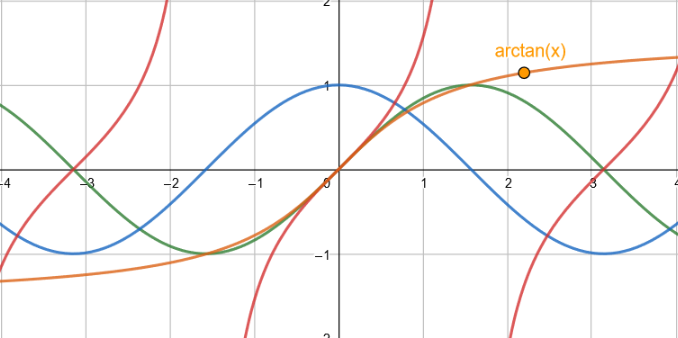
\includegraphics[width=\linewidth]{./bilder/winkelfunktionen.png}
\end{minipage}%
\hspace{0.01\linewidth}
\begin{minipage}{0.2\linewidth}
	\begin{tabular}[c]{ |c|c|c| }
		\hline
		arctan(x) & deg & rad \\
		\hline
		2-$\sqrt{3}$ & 0\symbol{23} & 0\\
		\hline
		$\sqrt{2}-1$ & 22.5\symbol{23} & $\frac{\pi}{8}$\\
		\hline
		$\frac{1}{\sqrt{3}}$ & 30\symbol{23} & $\frac{\pi}{6}$\\
		\hline
		1 & 45\symbol{23} & $\frac{\pi}{4}$\\
		\hline	
	\end{tabular}	
\end{minipage}
\hspace{0.01\linewidth}
\begin{minipage}{0.3\linewidth}
	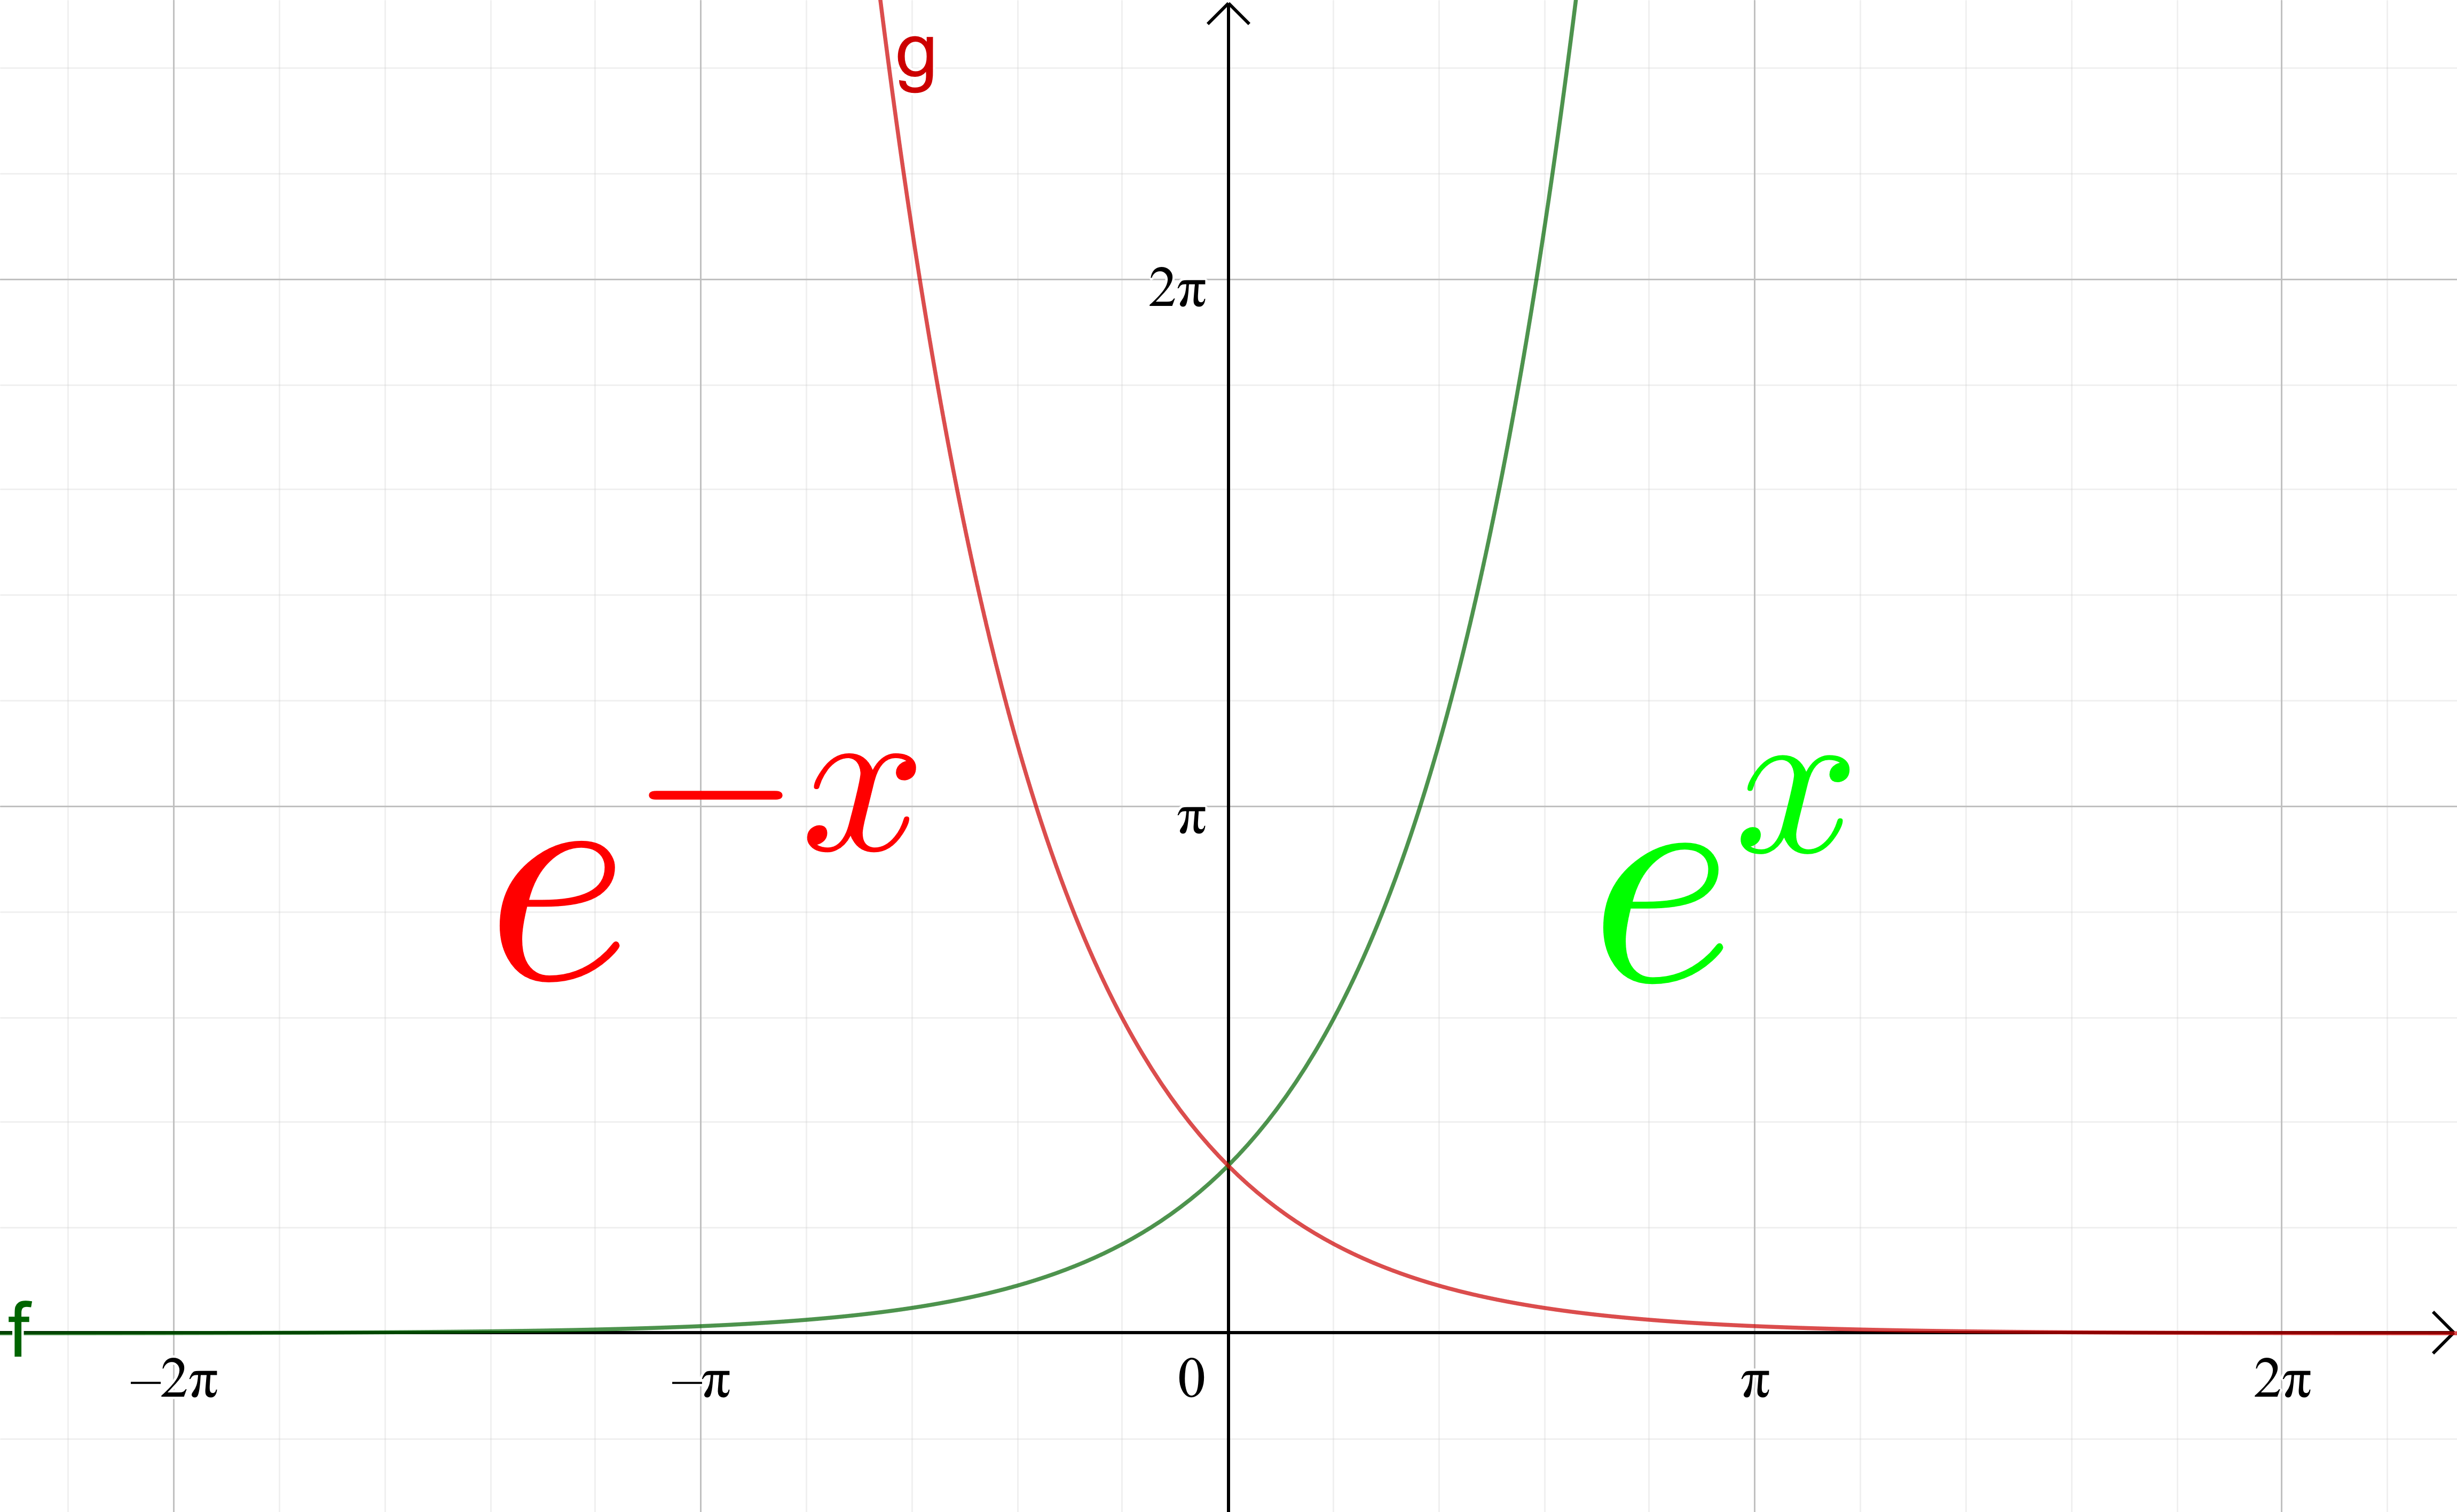
\includegraphics[width=\linewidth]{./bilder/e_kurven.png}
\end{minipage}


\begin{minipage}[t]{9cm}
	\subsection{Additionstheoreme}
	$\sin(a \pm b)=\sin(a) \cdot \cos(b) \pm \cos(a) \cdot \sin(b)$\\
	$\cos(a \pm b)=\cos(a) \cdot \cos(b) \mp \sin(a) \cdot \sin(b)$\\	
	$\tan(a \pm b)=\frac{\tan(a) \pm \tan(b)}{1 \mp \tan(a) \cdot \tan(b)}$
	
	\subsection{Doppel- und Halbwinkel}	
	$\sin(2a)=2\sin(a)\cos(a)$\\
	$\cos(2a)=\cos^2(a)-\sin^2(a)=2\cos^2(a)-1=1-2\sin^2(a)$\\
	$\cos^2 \left(\frac{a}{2}\right)=\frac{1+\cos(a)}{2} \qquad
	\sin^2 \left(\frac{a}{2}\right)=\frac{1-\cos(a)}{2}$
	
	\subsection{Produkte}
	$\sin(a)\sin(b)=\frac{1}{2}(\cos(a-b)-cos(a+b))$\\
	$\cos(a)\cos(b)=\frac{1}{2}(\cos(a-b)+cos(a+b))$\\
	$\sin(a)\cos(b)=\frac{1}{2}(\sin(a-b)+\sin(a+b))$	
\end{minipage}
\begin{minipage}[t]{6cm}
	\subsection{Quadrantenbeziehungen}
	\begin{tabbing}
		xxxxxxxxxxxxxxxxxxxxxxxxxxxxxxxxxx \= \kill
		$\sin(-a)=-\sin(a)$ \> $\cos(-a)=\cos(a)$\\
		$\sin(\pi - a)=\sin(a)$ \> $\cos(\pi - a)=-\cos(a)$\\
		$\sin(\pi + a)=-\sin(a)$ \> $\cos(\pi +a)=-\cos(a)$\\
		$\sin\left(\frac{\pi}{2}-a \right)=\sin\left(\frac{\pi}{2}+a \right)=\cos(a)$\\
		$\cos\left(\frac{\pi}{2}-a \right)=-\cos\left(\frac{\pi}{2}+a \right)=\sin(a)$  
	\end{tabbing}
	
	\subsection{Summe und Differenz}
	$\sin(a)+\sin(b)=2 \cdot \sin \left(\frac{a+b}{2}\right) \cdot
	\cos\left(\frac{a-b}{2}\right)$\\
	$\sin(a)-\sin(b)=2 \cdot \sin \left(\frac{a-b}{2}\right) \cdot
	\cos\left(\frac{a+b}{2}\right)$\\
	$\cos(a)+\cos(b)=2 \cdot \cos \left(\frac{a+b}{2}\right) \cdot
	\cos\left(\frac{a-b}{2}\right)$\\
	$\cos(a)-\cos(b)=-2 \cdot \sin \left(\frac{a+b}{2}\right) \cdot
	\cos\left(\frac{a-b}{2}\right)$\\
	$\tan(a) \pm \tan(b)=\frac{\sin(a \pm b)}{\cos(a)\cos(b)}$
\end{minipage}

%\subsection{Skalarprodukt}
%	\begin{tabular}{|p{3cm}|p{7cm}|p{7cm}|}
%	    \hline
%	    & Reelle Fourierreihe & Komplexe Fourierreihe \\
%	    \hline
%	    Skalarprodukt &  $\langle f;g \rangle = \frac{2}{T}\int\limits_0^Tf(t)\cdot
%	    g(t)\cdot dt $ & $\langle f;g \rangle = \frac{1}{T}\int\limits_0^Tf(t)\cdot
%	    \overline{g(t)}\cdot dt $ \\
%	    & $(I)\ \langle f;f \rangle > 0\ f"ur\ f\neq 0$ &
%	    $(I)\ \langle f;f \rangle > 0\ f"ur\ f\neq 0$ \\
%	    & $(II)\ \langle f;g \rangle = \langle g;f \rangle $ &
%	    $(II)\ \langle f;g \rangle = \overline{\langle g;f \rangle} $ \\
%	    & $(III) \langle r\cdot f;g\rangle = r\cdot\langle f;g\rangle,\ r\epsilon
%	    \mathbb R$ & $(III) \langle c\cdot f;g\rangle = c\cdot\langle f;g\rangle,\ 
%	    c\epsilon \mathbb R$
%	    \\
%	    \hline
%	    Länge (Norm): & \multicolumn{2}{|l|}{
%	    $\parallel f \parallel = \sqrt{\langle
%	    f;f \rangle} \Rightarrow y=3x^2+4 \rightarrow \sqrt{3\cdot3+4\cdot4}=5$ 
%	    } \\
%	    & \multicolumn{2}{|l|}{ $ (I)\ \parallel f \parallel > 0 f"ur f \neq 0$} \\
%	    & \multicolumn{2}{|l|}{ $ (II)\ \parallel f+g \parallel \leq \parallel f
%	    \parallel + \parallel g \parallel (Dreiecksgleichung)$} \\
%	    & \multicolumn{2}{|l|}{ $ (III)\ \parallel r\cdot f \parallel = |r| \cdot
%	    \parallel f \parallel , \ r \epsilon \mathbb R bzw. \parallel c\cdot
%	    f\parallel = |c|\cdot \parallel f \parallel, c\epsilon\mathbb C$} \\
%	    \hline
%	    Abstand: & \multicolumn{2}{|l|}{ $ \parallel f-g \parallel =
%	    |\sqrt{\langle f-g;f-g \rangle}| \Rightarrow
%	    |p-q|=(3x^2+4)-(x^2+7)=2x^2+11 \rightarrow
%	    \sqrt{2\cdot2+11\cdot11}=5\cdot\sqrt{5}$}
%	    \\
%	    \hline
%	    Winkel, Orthogonalit"at &
%	    \multicolumn{2}{|l|}{
%	    $\sphericalangle(f;g)=\arccos\left( \frac{\langle f;g \rangle}{\parallel f
%	    \parallel \cdot \parallel g \parallel} \right) = \arccos\left(\frac{\langle f;g 
%	    \rangle}{\sqrt{\langle f;f\rangle \cdot \langle g;g\rangle}}\right)$} \\
%	     & \multicolumn{2}{|l|}{$f \perp g\Leftrightarrow \langle f;g \rangle = 0$}
%	     \\
%	    
%	    
%	    \hline
%	\end{tabular}

\section{Diverses}
\begin{tabbing}
	xxxxxxxxxxxxxxxxxxxxxxxxxxxx \= xxxxxxxxxxxxxxxxxxxxxxxxxxxxxx \= \kill
	$f'(z) = \lim \limits_{\Delta z \rightarrow 0} \frac{f(z + \Delta z) -
		f(z)}{\Delta z}$ \> $(a + b)^n = \sum_{k=0}^{n} \binom n k a^{n-k} \cdot b^k$ \>
	$(a \pm b)^3 =a^3 \pm  3 a^{2} b + 3 a b^2 \pm b^3 $\\ \\
	$x_{1,2} = \frac{-b \pm \sqrt{b^2 - 4ac}}{2a}$ \> $\binom n k = \frac{n!}{k!
		\cdot (n-k)!}$ \> $(a \pm b)^4 =a^4 \pm  4 a^{3} b + 6a^2b^2 \pm 4 a b^3 +
	b^4$\\ 
\end{tabbing}

%\subsection{Integrale}
%	Partielle Integration: $\int^{b}_{a} u(x) v'(x) dx = [u(x)v(x)]^{b}_{a} - \int^{b}_{a} u'(x) v(x) dx$
%	\begin{center}
%	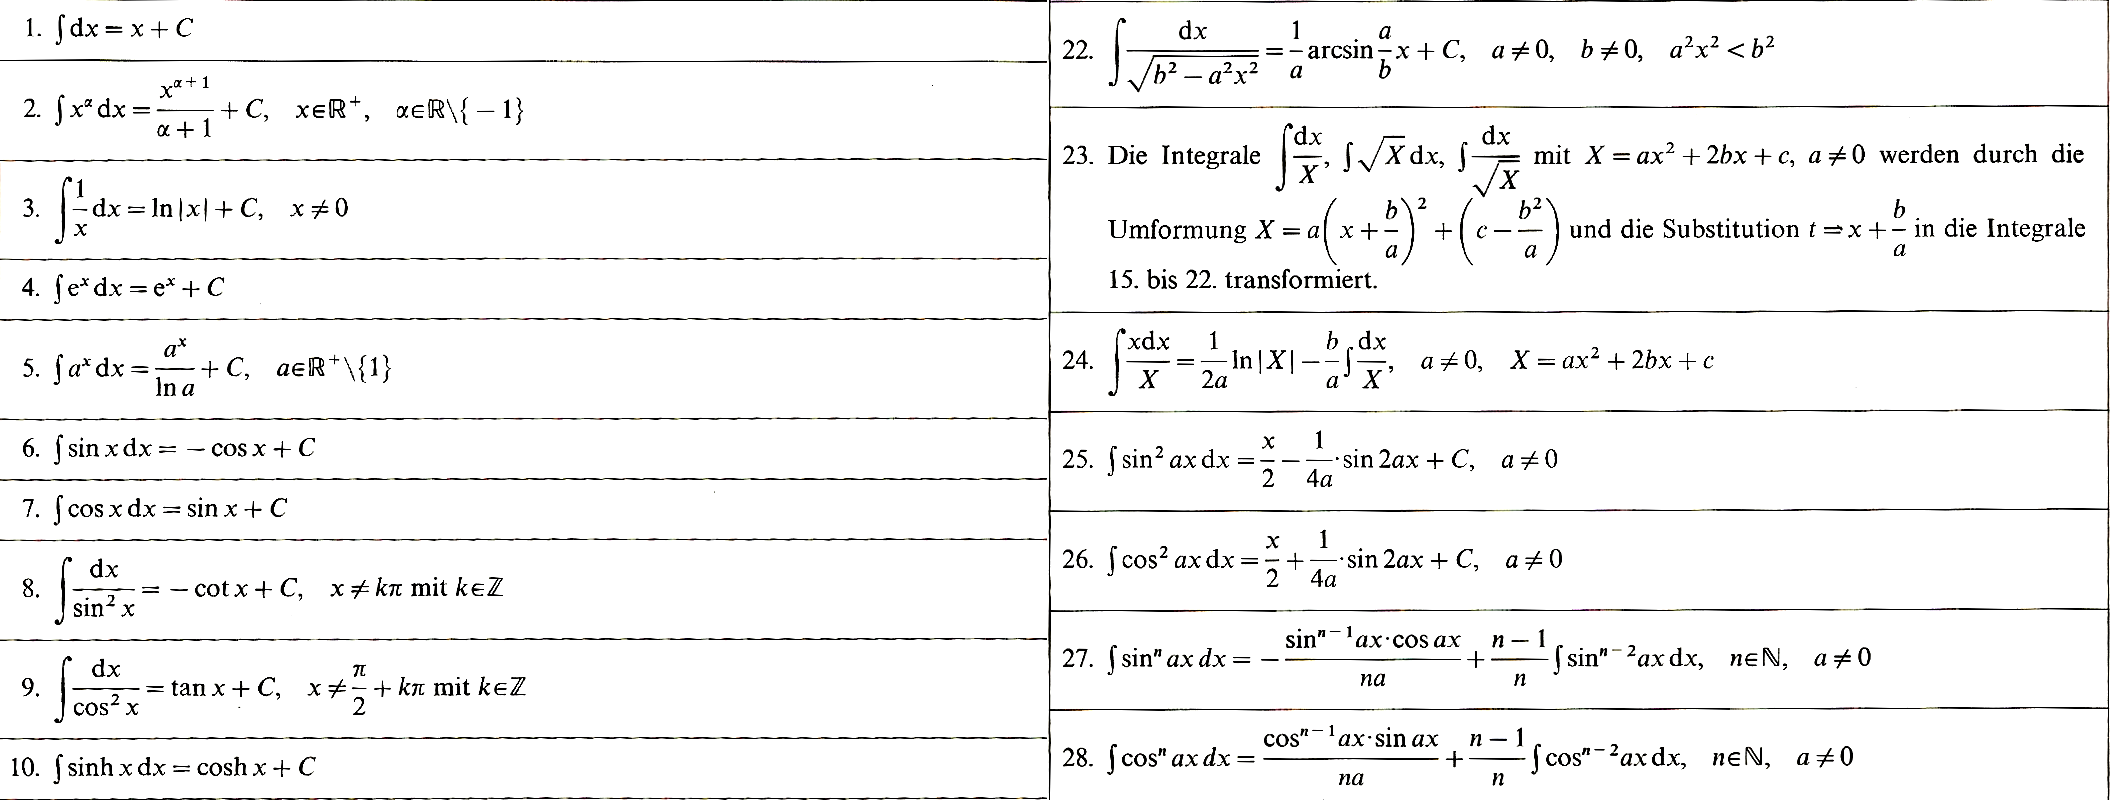
\includegraphics[width=\linewidth]{./bilder/integral1.png}
%	\end{center}
%	\begin{center}
%	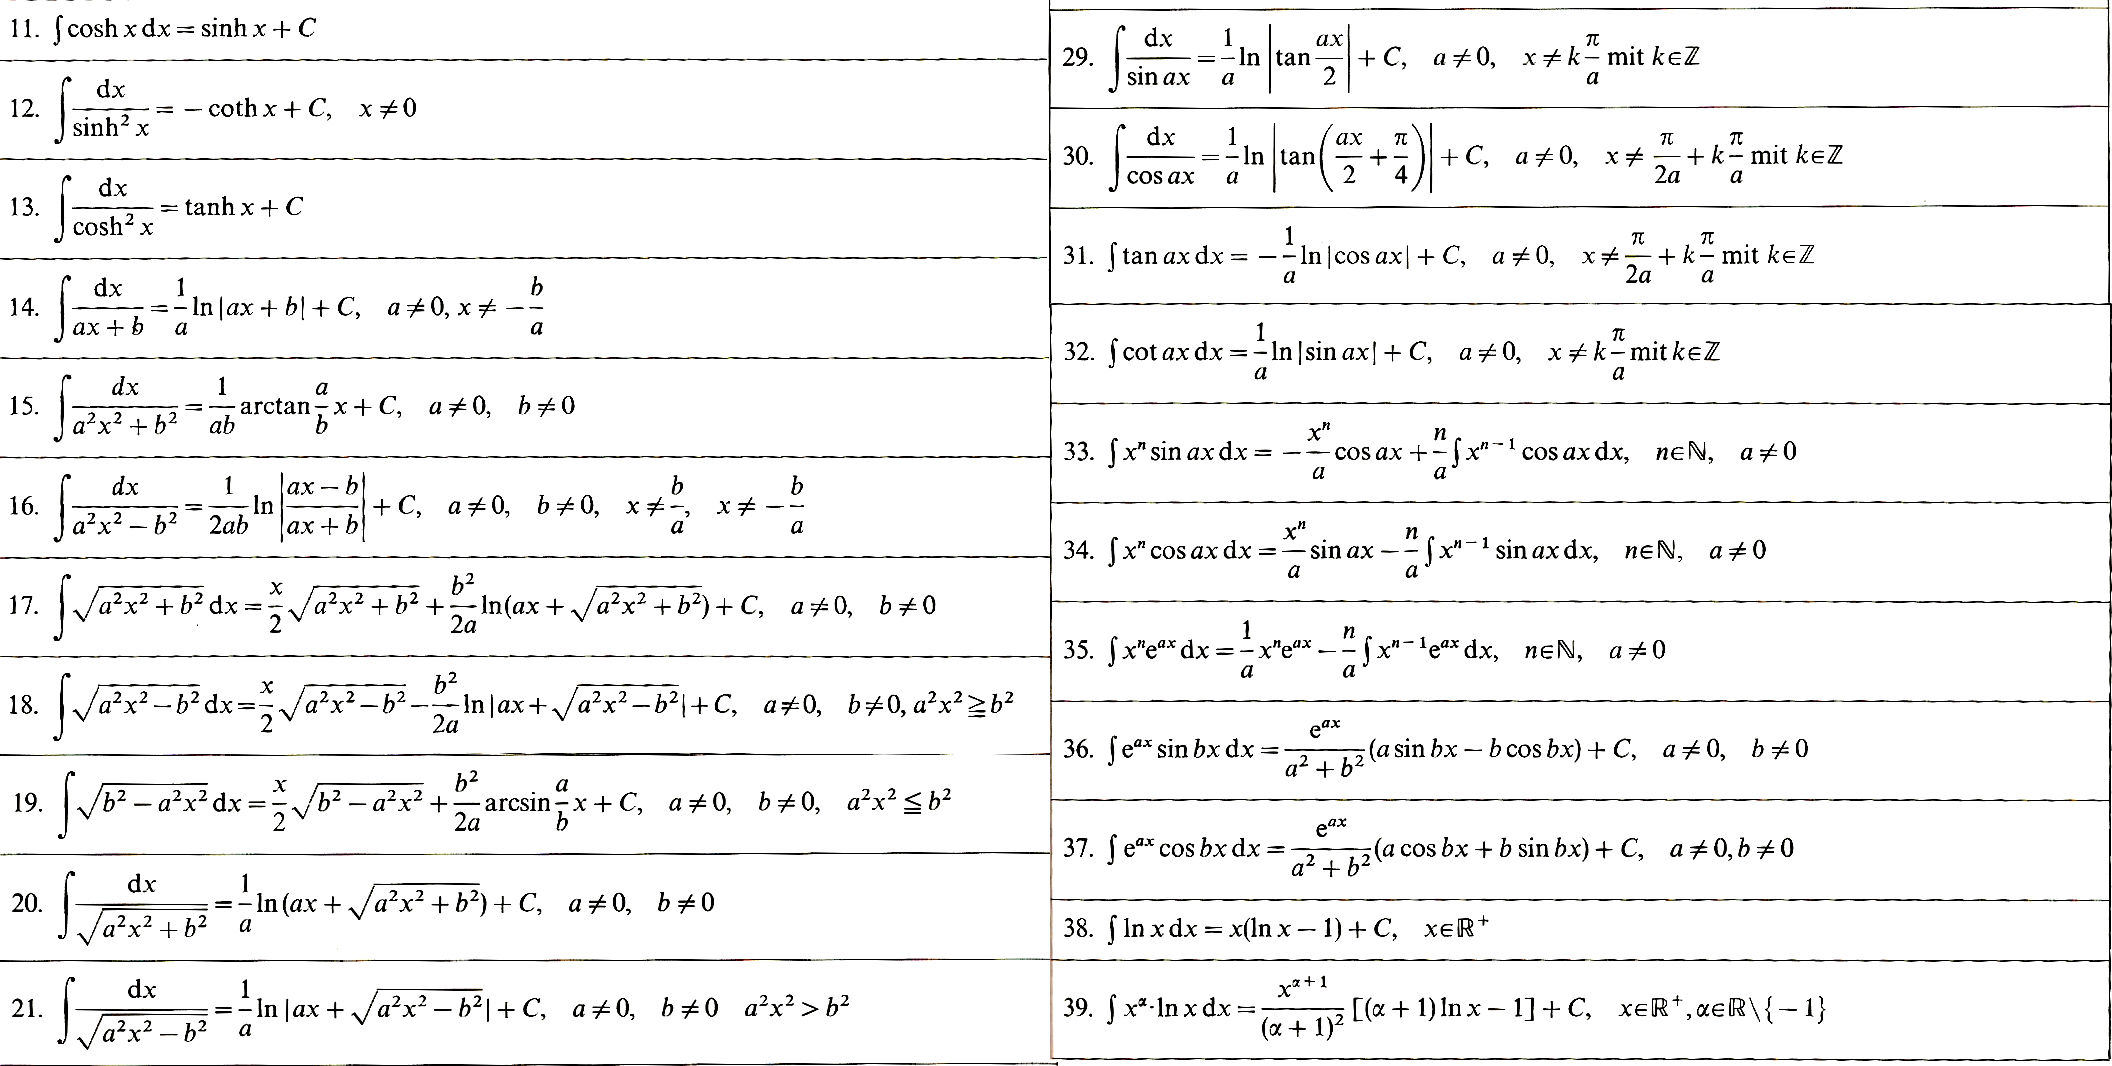
\includegraphics[width=\linewidth]{./bilder/integral2.png}
%	\end{center}

\section{Notizen}
\subsection{Gleichungen}
$arg(\frac{27}{(1+j)^8}) = arg(27) - arg((1+j)^8) = 2k\pi - 8\cdot arg(1+j) = 2k\pi -8(\frac{\pi}{4}+2l\pi) = 2k\pi - 2\pi - 16l\pi = 2\pi\overbrace{(k-8l-1)}^{m} = 2m\pi$\\ \vspace{\baselineskip}
$|e^{-j\frac{\pi}{6}}| = 1 (Betrag!)$\\ \vspace{\baselineskip}
$\frac{[cos(5) + j\cdot sin(5)]^6}{e^{j(30+40\pi)}} = \frac{[cjs(5)]^6}{e^{30j+40\pi j}} = \frac{(e^{5j})^6}{e^{30j}\cdot (e^{2\pi j})^{20}} = \frac{e^{30j}}{e^{30j}} = 1 $\\
------------------\\
$z^5 + z^3 + 8z^2 + 8 = 0 \rightarrow 0 = z^3(z^2 + 1) + 8(z^2 + 1) = (z^3 + 8)(z^2 + 1) \rightarrow z^3 + 8 = 0 \text{ oder }  z^2 + 1 = 0$\\
$z^3 + 8 = 0: z = \sqrt[3]{-8} = \sqrt[3]{|-8|}\cdot cjs(\frac{arg(-8)}{3} + k\frac{2\pi}{3}) = 2[cos(\frac{\pi}{3} + k\frac{2\pi}{3}) + j\cdot sin(\frac{\pi}{3} + k\frac{2\pi}{3})] \rightarrow k = 0 ...; k = 1 ...; k = 2 ...$\\
$z^2+1 = 0 : z^2 = -1 \rightarrow z = \sqrt{-1} \rightarrow z_4 = j; z_5 = -j$\\
------------------\\
$1 = \frac{e^z + e^{-z}}{2} \leftrightarrow 2 = e^z + e^{-z} \rightarrow{\cdot e^z}\rightarrow (e^z)^2 - 2e^z + 1 = 0 \rightarrow (e^z - 1)^2 = 0 \rightarrow e^z = 1 \rightarrow z = ln(1) + j\cdot (arg(1)+2k\pi) = j\cdot 2k\pi$\\
------------------\\
$\frac{e^{j\frac{a+b}{2}}}{2j} = \frac{e^{ja} + e^{jb}}{4j}   $



\subsection{Fourierreihen}
$c_n = \frac{1}{2\pi}\int\limits_{0}^{2\pi} sin(1.5t)\cdot e^{-jnt} dt -> \text{ Euler } -> \frac{1}{4\pi j} \int\limits_{0}^{2\pi} e^{(1.5-n)jt} - e^{(-1.5-n)jt} dt = \frac{1}{4\pi j}[\frac{e^{(1.5-n)jt
}}{(1.5-n)j}]_{0}^{2\pi} - \frac{1}{4\pi j} [\frac{e^{(-1.5-n)jt}}{(-1.5-n)j}]_{0}^{2\pi} = \frac{e^{3\pi j
}\cdot e^{-2\pi nj} -1}{-2(3-2n)\pi} + \frac{e^{-3\pi j} \cdot e^{-2\pi nj} -1}{-2(3+2n)\pi} = \frac{1}{(3-2n)\pi} + \frac{1}{(3+2n)\pi} = \frac{(3+2n) + (3-2n)}{(3-2n)(3+2n)\pi} = \frac{6}{(9-4n^2)\pi}$\\
------------------\\


\end{document}
